\documentclass[a4paper,11pt]{article}
%\usepackage{helvet}
%\renewcommand*\familydefault{\sfdefault}
%%% Language and font encodings
%\usepackage[english]{babel}
%\usepackage[utf8x]{inputenc}
%\usepackage[T1]{fontenc}

%% Sets page size and margins
%\usepackage[a4paper,top=3cm,bottom=2cm,left=3cm,right=3cm,marginparwidth=1.75cm]{geometry}
%\usepackage[a4paper,top=2cm,bottom=2cm,left=1.5cm,right=1.5cm,marginparwidth=1.75cm]{geometry}

\usepackage[margin=3cm]{geometry}
\usepackage{lineno}  % comment out for submissio

%% Useful packages
\usepackage[round]{natbib}
\usepackage[dvipsnames]{xcolor}
\usepackage{sectsty}
\usepackage{amsmath}
\usepackage{graphicx}
% \usepackage[colorinlistoftodos]{todonotes}
\usepackage[colorlinks=true, allcolors=blue]{hyperref}
%\usepackage{subfigure}
\usepackage{soul} % strikethrough
% \usepackage{floatrow}  % causes conflicts
\usepackage{hyperref}
\usepackage{csquotes}
\usepackage[bf,font=small]{caption}

\sectionfont{\color{Mahogany}}
\subsectionfont{\color{Mahogany}}

%% Left justified title
%\usepackage{etoolbox}
%\makeatletter
%\patchcmd{\@maketitle}{\begin{center}}{\begin{flushleft}}{}{}
%\patchcmd{\@maketitle}{\begin{tabular}[t]{c}}{\begin{tabular}[t]{@{}l}}{}{}
%\patchcmd{\@maketitle}{\end{center}}{\end{flushleft}}{}{}
%\makeatother

% Supplement
\newcommand{\beginsupplement}{%
        \setcounter{table}{0}
        \renewcommand{\thetable}{S\arabic{table}}%
        \setcounter{figure}{0}
        \renewcommand{\thefigure}{S\arabic{figure}}%
     }

%\title{\textbf{Why deconvolve Ca\textsuperscript{2+}? \\ \large A practical guide to recovering neural activity from cellular fluorescence imaging}}
\title{\textbf{On the use of calcium deconvolution algorithms in practical contexts}}

\author{Mathew H. Evans$^{1,2}$, Rasmus S. Petersen$^2$ \& Mark D. Humphries$^{1,2}$}
\date{%
    $^1$School of Psychology, University of Nottingham, UK\\%
    $^2$Faculty of Biology, Medicine and Health, University of Manchester, UK\\[2ex]%
    \today
}

\begin{document}
\maketitle

\linenumbers
\begin{abstract}
Calcium imaging is a powerful tool for capturing the simultaneous activity of large populations of neurons. Studies using it to address scientific questions of population dynamics and coding often use the “raw” time-series of changes in calcium fluorescence at the soma. But somatic calcium traces are both contaminated with multiple noise sources and are non-linearly related to spiking. A suite of methods are available to recover spike-evoked events from the raw calcium, from simple deconvolution to inferring the spikes themselves. Here we explore the extent to which our choice of raw or deconvolved calcium time-series affects the scientific inferences we can draw. Our results show the choice qualitatively changes the potential scientific inferences we draw about neural activity, coding, and correlation structure. We show that a substantial fraction of the processing methods fail to recover simple features of population activity in barrel cortex already established by electrophysiological recordings. Raw calcium time-series contain an order of magnitude more cells tuned to task features; yet there is also qualitative disagreement between deconvolution methods on which neurons are tuned. Finally, we show that raw and processed calcium time-series qualitatively disagree on the structure of correlations within the population and the dimensionality of its joint activity. We suggest that quantitative results obtained from population calcium-imaging be verified across multiple forms of the calcium time-series. 
\end{abstract}


\section{Introduction}
Calcium imaging is a wonderful tool for high yield recordings of large neural populations \citep{Harris2016-zo, Stringer2019-ze,  Ahrens2013-wm, Portugues2014-kq}. Many pipelines are available for moving from pixel intensity across frames of video to a time-series of calcium fluorescence in the soma of identified neurons \citep{Mukamel2009-am, Vogelstein2010-uc, Kaifosh2014-zo, Pachitariu2016-ui, Deneux2016-gu, Pnevmatikakis2016-tk, Friedrich2017-ym, Keemink2018-li, Giovannucci2019-nj}.

But raw calcium fluorescence is nonlinearly related to spiking, and contains noise from a range of sources. These issues have inspired a wide range of deconvolution algorithms \citep{Theis2016-ee, Berens2018-su, Stringer2018-st}, which attempt to turn raw somatic calcium into something more closely approximating spikes. We address here the question facing any systems neuroscientist using calcium imaging: do we use the raw calcium, or attempt to clean it up? Thus our aim is to understand if our choice matters: how do our scientific inferences depend on our choice of raw or deconvolved calcium time-series.

Deconvolution algorithms themselves range in complexity from simple deconvolution with a fixed kernel of the calcium response \citep{Yaksi2006-ic}, through detecting spike-evoked calcium events \citep{Jewell2018-cx, Pachitariu2016-ui}, to directly inferring spike times \citep{Vogelstein2010-uc, Lutcke2013-wu, Deneux2016-gu}. This continuum of options raise the further question of the extent to which we should process the raw calcium signals. 

We proceed in two stages. In order to use deconvolution algorithms, we need to choose their parameters. We’d like to know whether it is worth taking this extra step: how good can these algorithms be in principle, and how sensitive their results are to the choice of parameter values. We thus first evaluate qualitatively different deconvolution algorithms, by optimising their parameters against ground truth data with known spikes. With our understanding of their parameters in hand, we then turn to our main question, by analysing a large-scale population recording from the barrel cortex of a mouse performing a whisker-based decision task. We compare the scientific inferences about population coding and correlations we obtain using either raw calcium signals, or a range of time-series derived from those calcium signals, covering simple deconvolution, event detection, and spikes. 

We find contrasting answers. A substantial fraction of the methods used here fail to recover basic features of population activity in barrel cortex established from electrophysiology. The inferences we draw about coding qualitatively differ between raw and deconvolved calcium signals. In particular, coding analyses based on raw calcium signals detect an order of magnitude more cells tuned to task features. Yet there is also qualitative disagreement between deconvolution methods on which neurons are tuned. The inferences we draw about correlations between neurons do not distinguish between raw and deconvolved calcium signals, but can qualitatively differ between deconvolution methods. Our results thus suggest care is needed in drawing inferences from population recordings of somatic calcium, and that one solution is to replicate all results in both raw and deconvolved calcium signals.

\section{Results} 
\subsection{Performance of deconvolution algorithms on ground-truth data-sets}\label{GT}
We select here three deconvolution algorithms that infer discrete spike-like events, each an example of the state of the art in qualitatively different approaches to the problem: Suite2p \citep{Pachitariu2016-ui}, a peeling algorithm that matches a scalable kernel to the calcium signal to detect spike-triggered calcium events; LZero \citep{Jewell2018-cx}, a change-point detection algorithm, which finds as events the step-like changes in the calcium signal that imply spikes; and MLspike \citep{Deneux2016-gu}, a forward model, which fits an explicit model of the spike-to-calcium dynamics in order to find spike-evoked changes in the calcium signal, and returns spike times. We emphasis that these methods were chosen as exemplars of their approaches, and are each innovative takes on the problem; we are not here critiquing individual methods, but using an array of methods to illustrate the problems and decisions facing the experimentalist when using calcium imaging data.

We first ask if these deconvolution methods work well in principle. We fit the parameters of each method to a data-set of 21 ground-truth recordings \citep{Chen2013-nv}, where the spiking activity of a cell is recorded simultaneously with 60 Hz calcium imaging using high-signal-to-noise juxtacellular recording techniques (Figure \ref{fig:GT_data}a). To fit the parameters for each recording, we sweep each method's parameter space to find the parameter value(s) with the best match between the true and inferred spike train. 

\begin{figure}
	\centering
	% \floatbox[{\capbeside\thisfloatsetup{capbesideposition={right,top},capbesidewidth=0.4\textwidth}}]{figure}[\FBwidth]	
	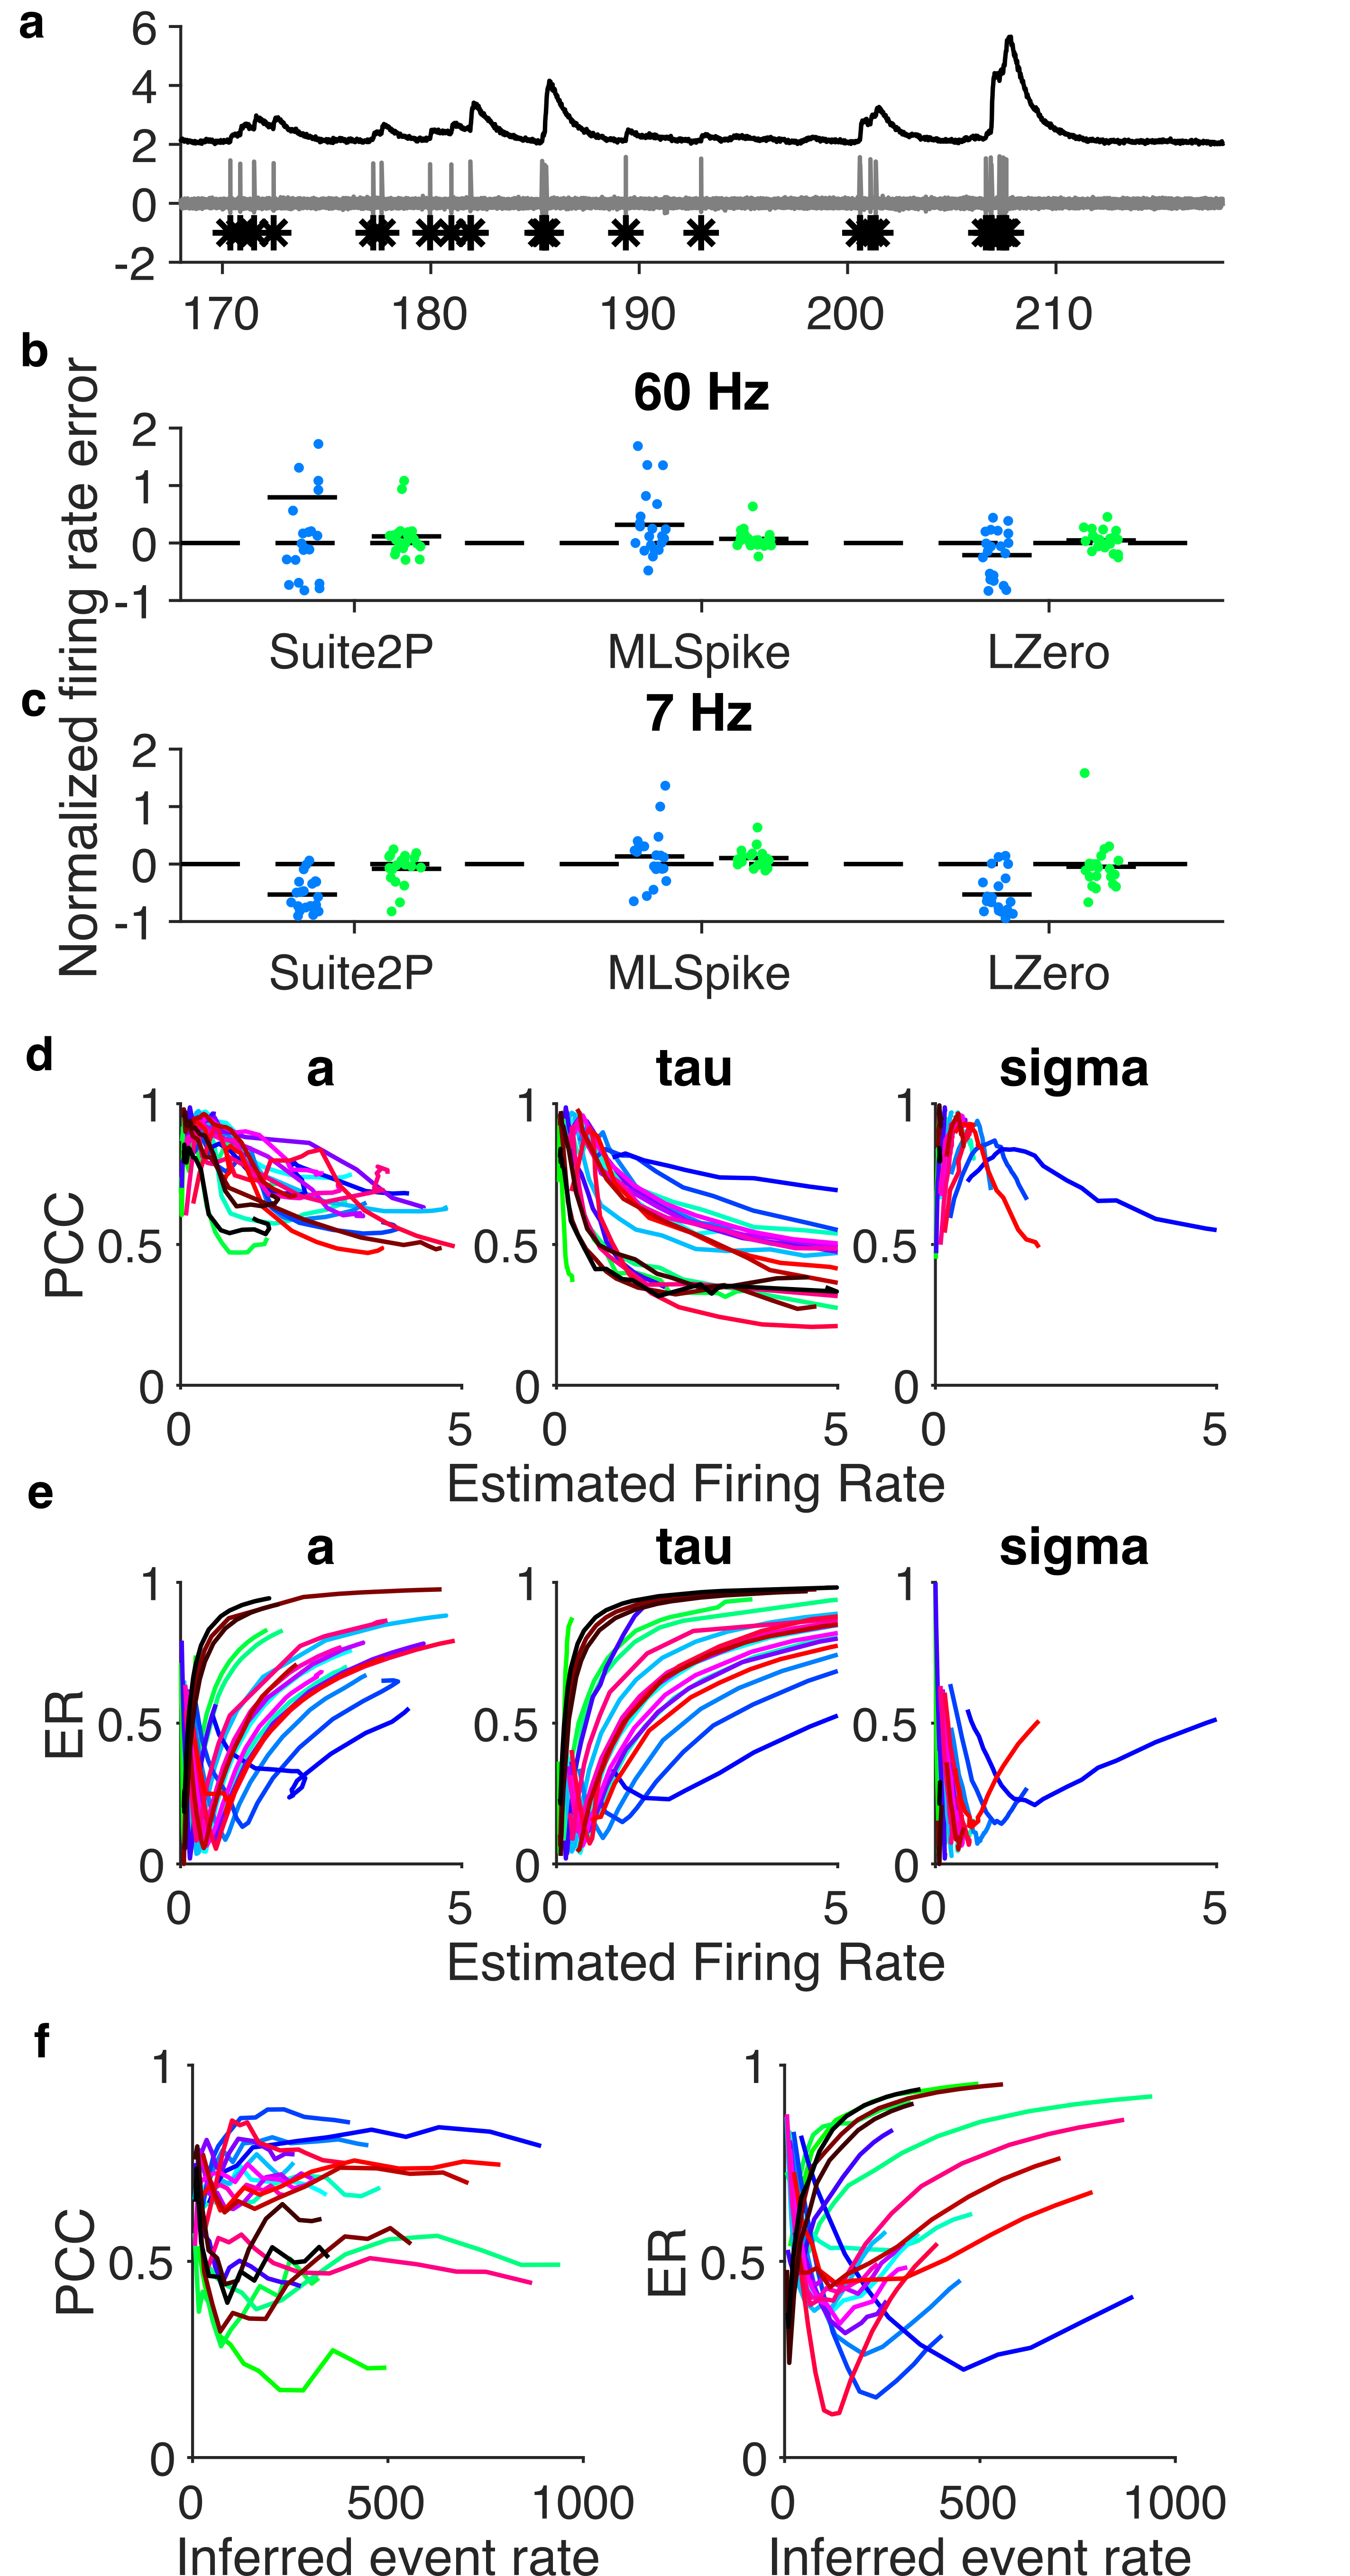
\includegraphics[width=0.5\textwidth]{composite_figs/fig1_ground_truth.png}
	\caption{\textbf{Ground truth data analysis.} \label{fig:GT_data} \\
		(a) Example simultaneous recording of somatic voltage (grey) and calcium activity (black) imaged at 60Hz. Spikes are marked with asterisks. \\ 
		(b) Error in estimating the true firing rate when using optimised parameters, across all three methods. One symbol per recording. We separately plot errors for parameters optimised to maximise the correlation coefficient (PCC), the errors for parameters optimised to minimise the error rate (ER). Horizontal black bars are means. Error is computed relative to the true firing rate: $(Rate_{true} - Rate_{estimated} / Rate_{true})$. For LZero and Suite2p, $Rate_{estimated}$ is computed from event times.  \\
		(c) As for (b), but with the somatic calcium down-sampled to 7Hz before optimising parameters for the deconvolution methods. \\
		(d) Dependence of MLspike's deconvolution performance on the firing rate of the inferred spike train. For each of MLSpike's free parameters, we plot the correlation coefficient between true and inferred spikes as a function of the firing rate estimated from the inferred spikes. One line per recording. Parameters: $A$: calcium transient amplitude per spike ($\Delta F/F$); $\tau$ calcium decay time constant (s); $\sigma$: background (photonic) noise level ($\Delta F/F$)\\
		(e) as in (d), but using Error Rate between the true and inferred spikes. \\
		(f) Dependence of Suite2p's deconvolution performance on the firing rate of the inferred event train as a detection threshold parameter is varied. Left: correlation coefficient; right: Error Rate.
		% (d) Comparison of estimated firing rates for the optimised  parameters against the true firing rate for each neuron. For each spike deconvolution method, we plot two estimated firing rates per recording (linked symbols), one for parameters optimised to maximise the correlation coefficient (PCC), the other for parameters optimised to minimise the error rate (ER). \\ 
	}
\end{figure}

The best-fit parameters depend strongly on how we evaluate the match between true and inferred spikes. The Pearson correlation coefficient between the true and inferred spike train is a common choice \citep{Brown2004-tj, Paiva2010-qv,Theis2016-ee, Reynolds2018-yh, Berens2018-su}, typically with both trains convolved with a Gaussian kernel to allow for timing errors. However, we find that choosing parameters to maximise the correlation coefficient can create notable errors. The inferred spike trains from MLSpike have too many spikes on average (mean error: 31.72$\%$), and the accuracy of recovered firing rates widely varies across recordings (Fig \ref{fig:GT_data}b, blue symbols). We attribute these errors to the noisy relationship between the correlation coefficient and the number of inferred spikes (Figure \ref{fig:GT_data}c): for many recordings, there is no well-defined maximum coefficient, especially for the amplitude parameter $A$, so that near-maximum correlation between true and inferred trains is consistent with a wide range of spike counts in the inferred trains. We see the same sensitivity for the event rates from recordings optimised using Suite2p (Figure \ref{fig:GT_data}f). If we compare their inferred event rates to true firing rates (Fig \ref{fig:GT_data}b), we see Suite2p estimates far more events than spikes (mean error 79.47$\%$) and LZero fewer events than spikes (mean error: -21.14$\%$). These further errors are problematic: there cannot be more spike-driven calcium events than spikes, and LZero's underestimate is considerably larger than the fraction of frames with two or more spikes ($<$2e$^{-4}\%$ frames).  

To address the weaknesses of the Pearson correlation coefficient, we instead optimise parameters using the Error Rate metric of \citet{Deneux2016-gu}. Error Rate returns a normalised score between 0 for a perfect match between two spike trains, and 1 when all the spikes are missed. This comparison between inferred and true spike trains is most straightforward for algorithms like MLSpike that directly return spike times; for the other algorithms, we use here their event times as inferred spikes, a reasonable choice given the low firing rate and well separated spikes in the ground truth data. Choosing parameters to minimise the Error Rate between the true and inferred spike-trains results in excellent recovery of the true number of spikes for all three deconvolution methods (Fig \ref{fig:GT_data}b, green symbols), with mean errors of 12$\%$ for Suite2P, 7.3$\%$ for MLSpike, and 5$\%$ for LZero. As we show in Figure \ref{fig:GT_data}e for MLSpike and Figure \ref{fig:GT_data}f for Suite2p, the Error Rate has a well-defined minima for almost every recording. Consequently, all deconvolution methods can, in principle, accurately recover the true spike-trains given an appropriate choice of parameters.

A potential caveat here is that the ground-truth data are single neurons imaged at a frame-rate of 60Hz, an order of magnitude greater than is typically achievable in population recordings \citep{Peron2015-qz}. Such a high frame-rate could allow for more accurate recovery of spikes than is possible in population recordings. To test this, we downsample the ground-truth data to a 7Hz frame-rate, and repeat the parameter sweeps for each deconvolution method applied to each recording. As we show in Figure \ref{fig:GT_data}c, optimising parameters using the minimum Error Rate still results in excellent recovery of the true spike rate (and interestingly for some recordings reduces the error when using the correlation coefficient). Lower frame-rates need not then be an impediment to using deconvolution methods. 

\subsection{Parameters optimised on ground-truth are widely distributed and sensitive}

What might be an impediment to using deconvolution methods on population recordings is that the best parameter values vary widely between cells. Figure \ref{fig:GT_data_params}a-b plots the best-fit parameter values for each recording across deconvolution methods and sampling rates. Each method has at least one parameter with substantial variability across recordings, varying by an order of magnitude or more. This suggests that the best parameters for one cell may perform poorly for another cell.

\begin{figure}[h!]
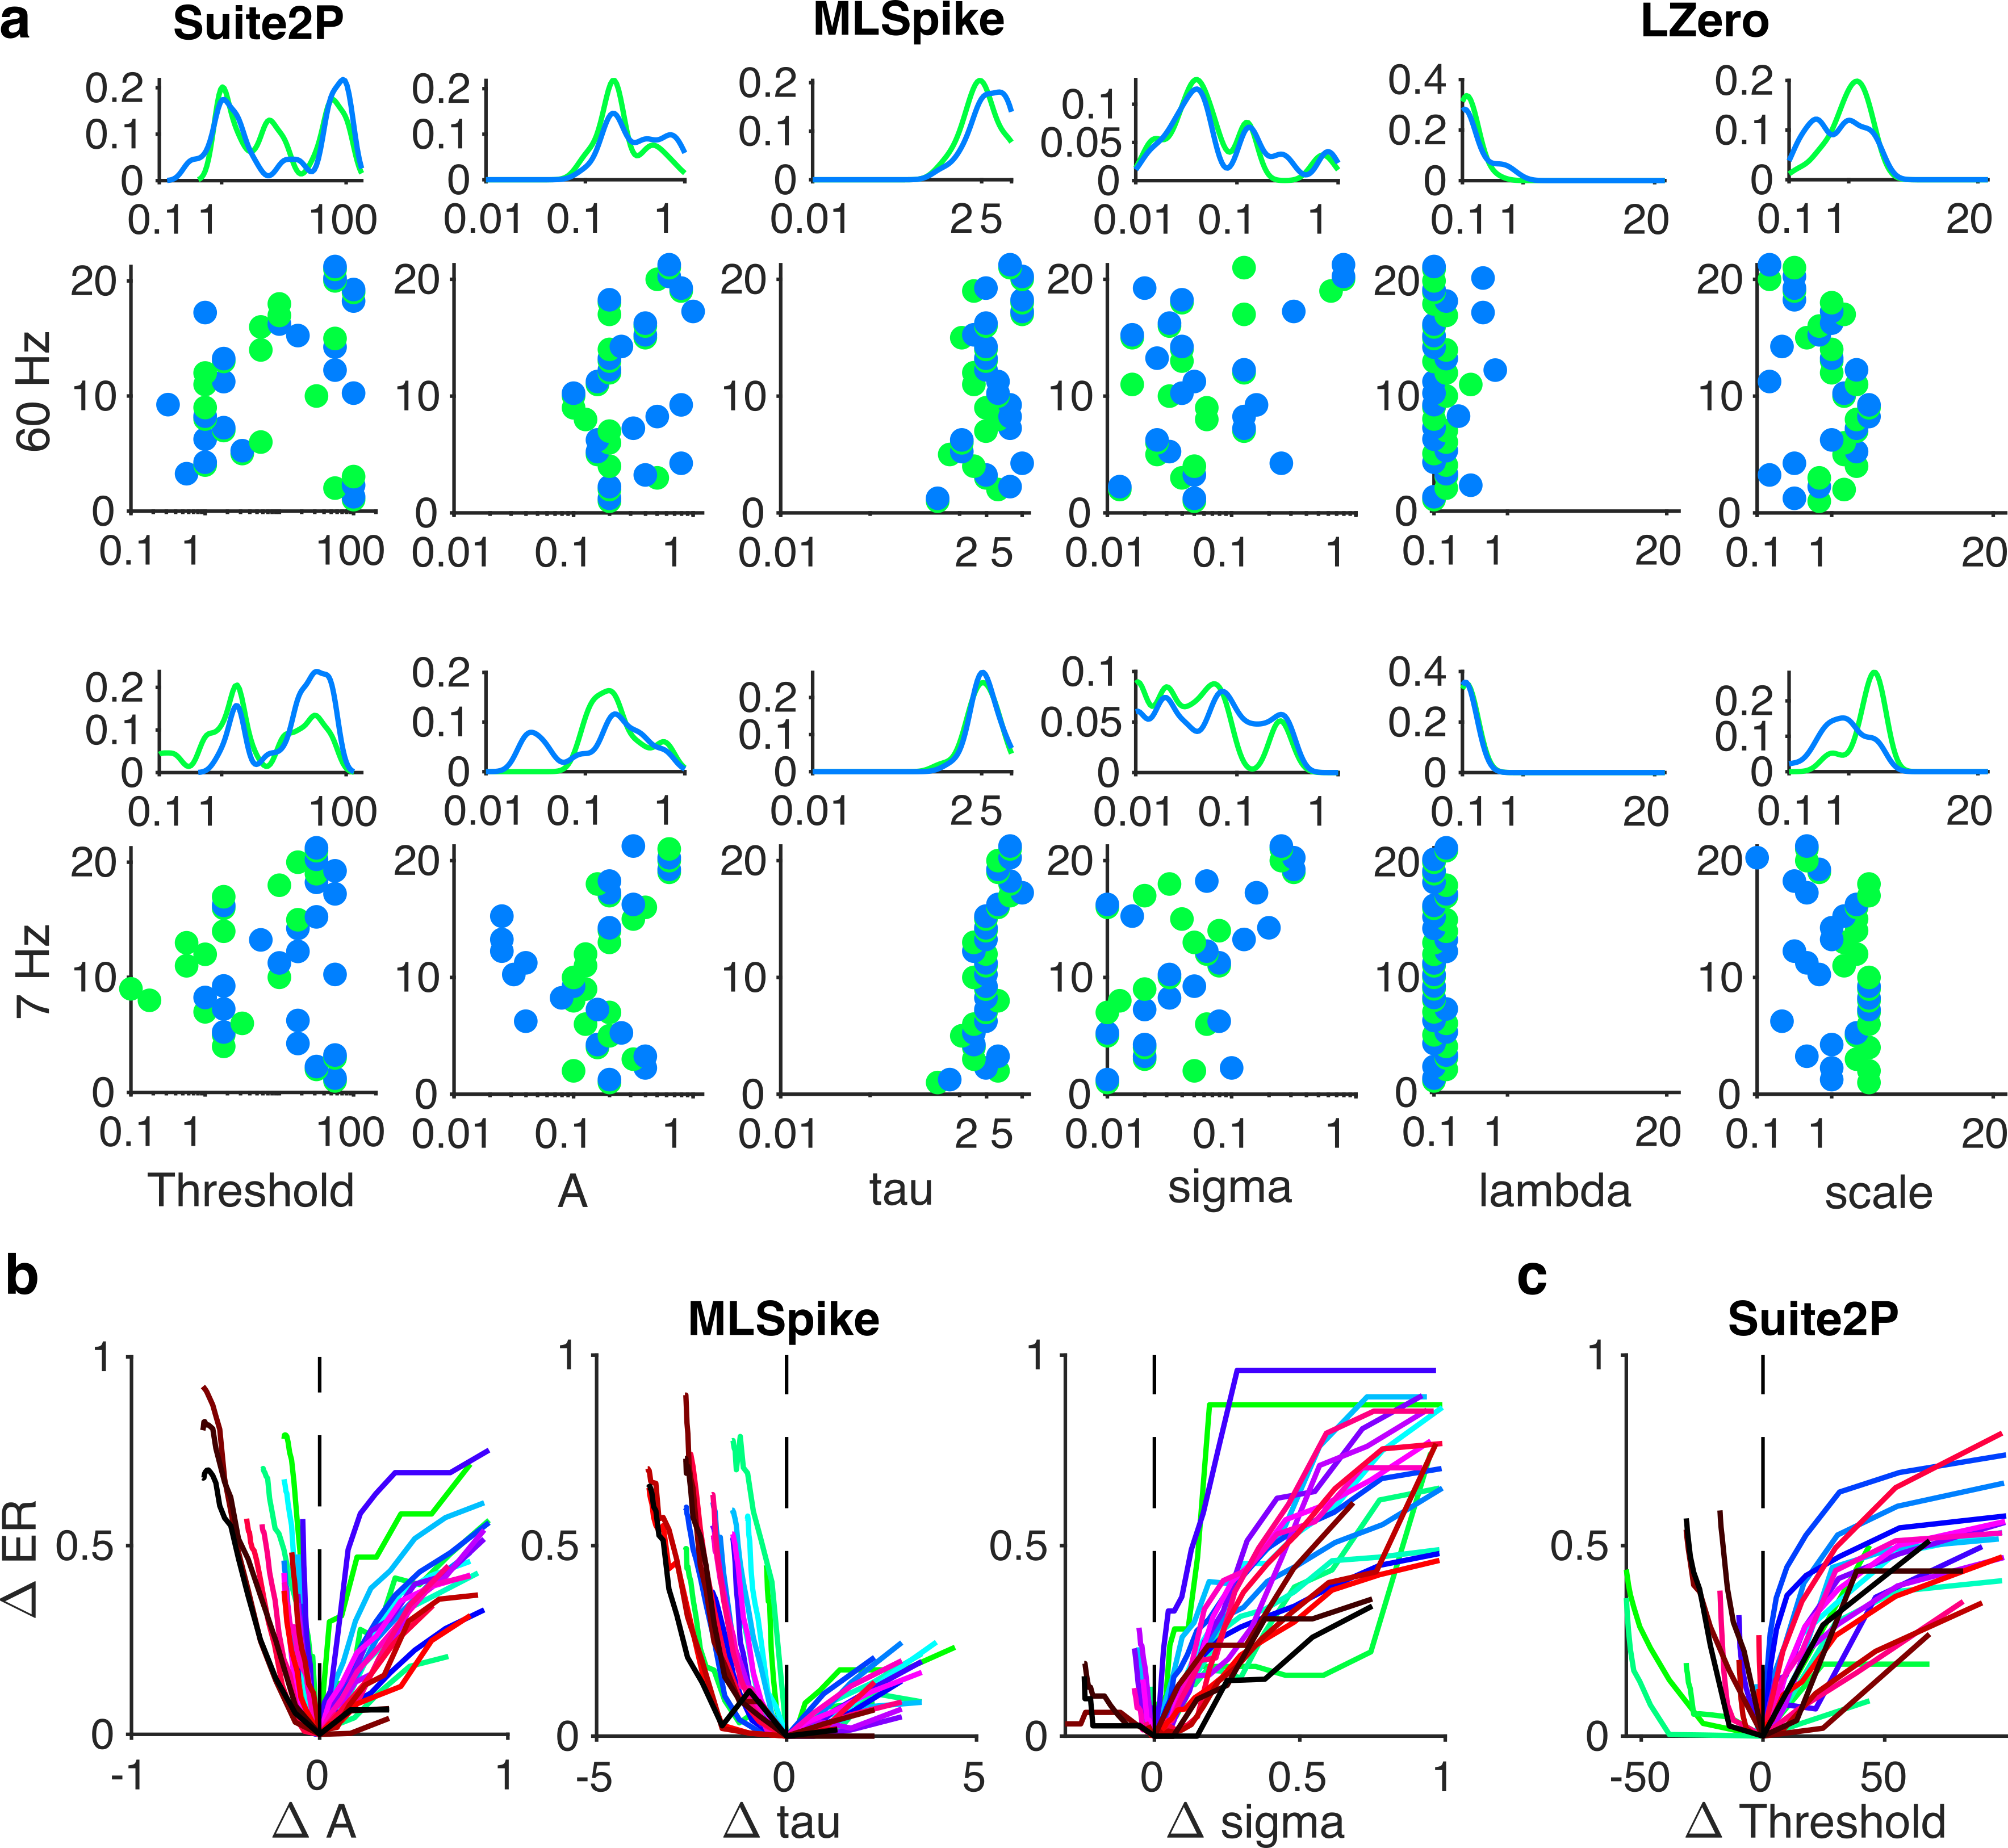
\includegraphics[width=\textwidth]{composite_figs/fig2_param_sweep.png}
\caption{\textbf{Variation in best-fit spike deconvolution parameters across ground-truth recordings.} 	\label{fig:GT_data_params} \\
	(a) Distributions of optimised parameter values across recordings. In each panel, we plot parameter values on the x-axis against the recording ID on the y-axis (in an arbitrary but consistent order). Parameter values are plotted for those optimised using the Error Rate (green). Top row: fits to the original 60 Hz frame-rate data; bottom row: fits to data down-sampled to 7 Hz.  [1: link recordings of the same cell {\color{red} what do you mean? Each cell is in its own y-axis position already, so horizontal lines between blue and green dots?}] \\
	(b) Change in error rate as a function of the change away from a parameter's optimum value, for each of MLSpike's free parameters. One line per recording. \\
	(c) Change in the error rate with change in Suite2p's threshold value away from its optimum for each recording. One line per recording.
	% (e) [Quantify (f) for all 3 methods, for all parameters: what is slope of ER change from minima with variation? [e.g. Take approx derivative]]
}
\end{figure}

The problem of between-cell variation in parameter values would be compensated somewhat if the quality of the inferred spike or event trains is robust to changes in those values. However, we find performance is highly sensitive to changes in some parameters. Figure \ref{fig:GT_data_params}b-c shows that for most recordings the quality of the inferred spike train abruptly worsens with small increases or decreases in the best parameter. Thus using deconvolution algorithms on population recordings comes with the potential issues that parameters can be both sensitive and vary considerably across cells.


\subsection{Deconvolution of population imaging in barrel cortex during a decision task}
We turn now to seeing if and how these issues play out when analysing a large-scale population recording with no ground-truth. The data we use are two-photon calcium imaging time-series from a head-fixed mouse performing a whisker-based two-alternative decision task (Fig. \ref{fig:peron_setup}a-b), from the study of \citet{Peron2015-kd}. We analyse here a single session with 1552 simultaneously recorded pyramidal neurons in L2/3 of a single barrel in somatosensory cortex, imaged at 7 Hz for just over 56 minutes, giving 23559 frames in total across 335 trials of the task. 

\begin{figure}[h!]
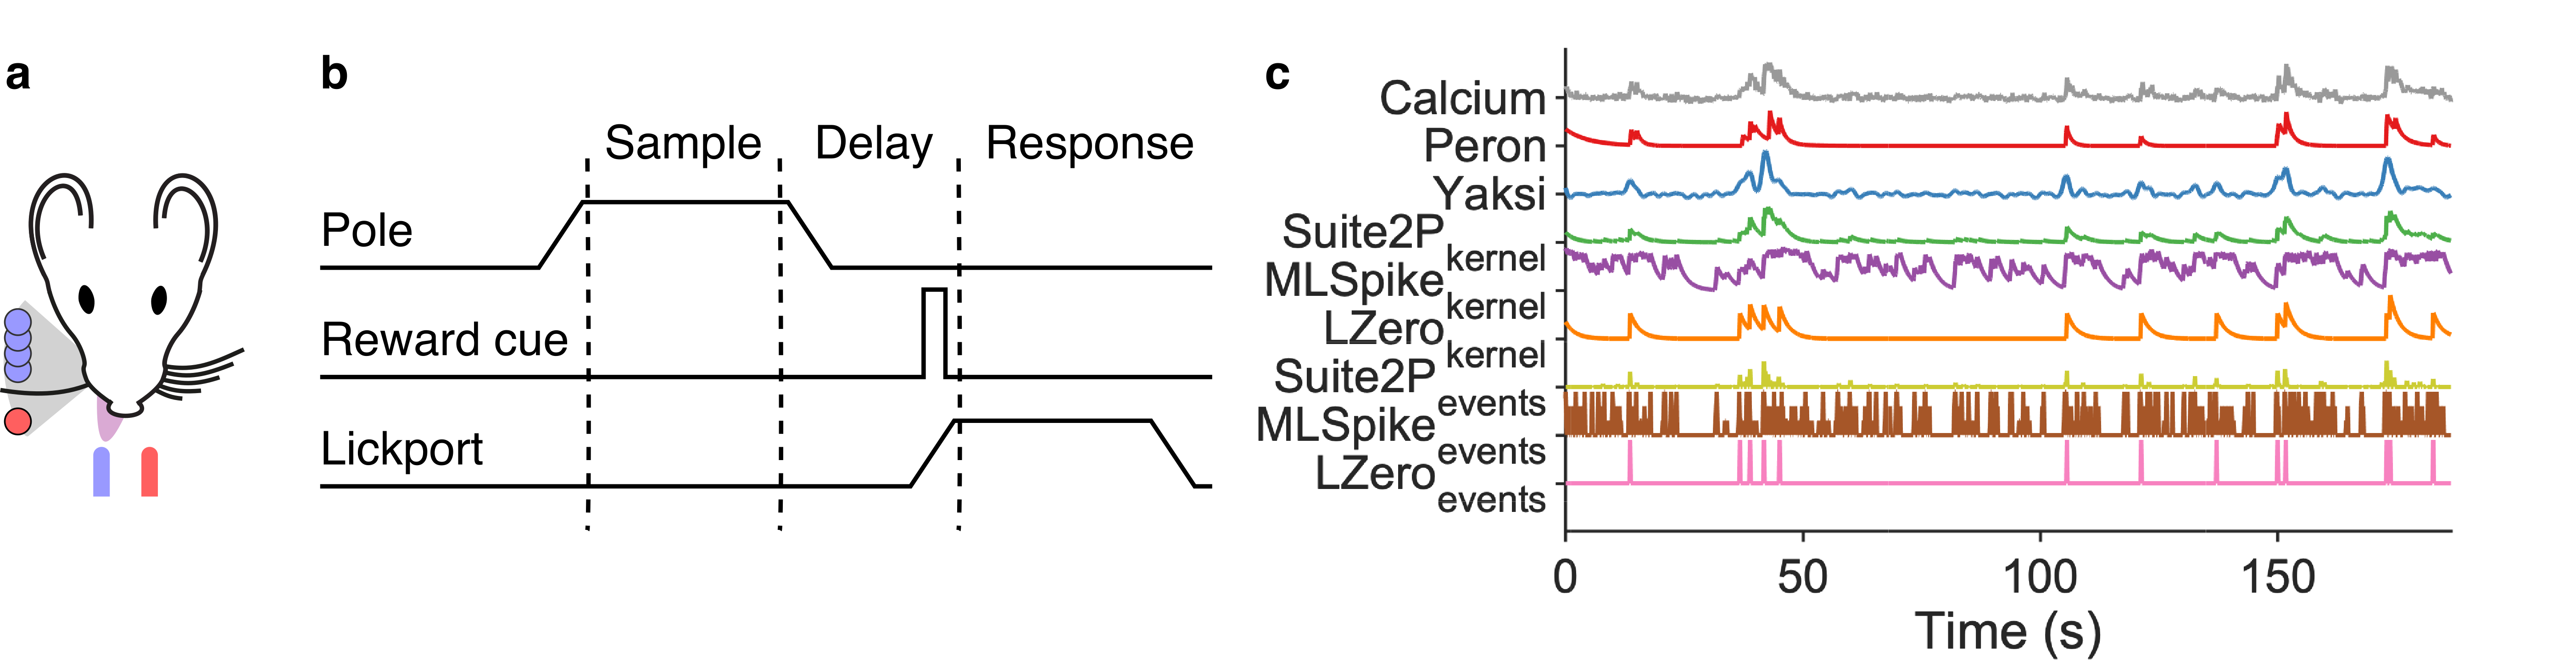
\includegraphics[width=\textwidth]{composite_figs/fig3_schematic.png}
    \caption{\label{fig:peron_setup} \textbf{Experimental data from \citet{Peron2015-kd}}. \\
		(a) Schematic of task set-up. A pole was raised within range of the single left-hand whisker; its position, forward (red) or backward (blue) indicated whether reward would be available from the left or right lick-port. \\
		(b) Schematic of trial events. The pole was raised and lowered during the sample period; a auditory cue indicated the start of the response period. \\
		(c) All deconvolution methods applied to one raw calcium signal from the same neuron.}
\end{figure}

Our primary goal is to understand how the choices of deconvolving these calcium-imaging data alter the scientific inferences we can draw.  As our baseline, we use the ``raw'' $\Delta F/F$ time-series of changes in calcium indicator fluorescence. We use the above three discrete deconvolution methods to extract spike counts (MLSpike), event occurrence (LZero), or event magnitude (Suite2p) per frame. For comparison, we use \citet{Peron2015-kd}'s own version of denoised calcium time-series, created using a custom version of the peeling algorithm \citep{Lutcke2013-wu}, a greedy template-fitting algorithm with variable decay time constants across events and cells, with parameters chosen to result in the same proportion of silent cells as has been shown previously with unbiased electrophysiology. As an example of simpler methods, we use \citet{Yaksi2006-ic}'s simple deconvolution of the raw calcium with a fixed kernel of the calcium response to a single spike. And finally we create smoothed versions of the discrete-deconvolution methods, by convolving their recovered spikes/events with a fixed spike-response kernel. Figure \ref{fig:peron_setup}c show an example raw calcium time-series for one neuron, and the result of applying each of these 8 processing methods. We thus repeat all analyses on 9 different sets of time-series extracted from the same population recording. 

We choose the algorithm parameters as follows. Simple deconvolution \citep{Yaksi2006-ic} involves taking a parameterised kernel of the GCaMP6s response to a single spike [Same as Peron’s kernel? {\color{red} no, Peron used a bank of kernels. The kernel matches Suite2P's default GCaMP6s kernel, and the one used in LZero's internal cost function}]. For the three discrete deconvolution methods, we choose the modal values of the best-fit parameters that optimised the Error Rate over the ground-truth recordings. This seems a reasonably consistent choice, of using the most consistently performing values obtained from comparable data: neurons in the same layer (L2/3) in the same species (mouse), in another primary sensory area (V1). Most importantly for our purposes, choosing the modal values means we avoid pathological regions of the parameter space.


\subsection{Deconvolution methods disagree on estimates of simple neural statistics}
\begin{figure*}
	\centering
	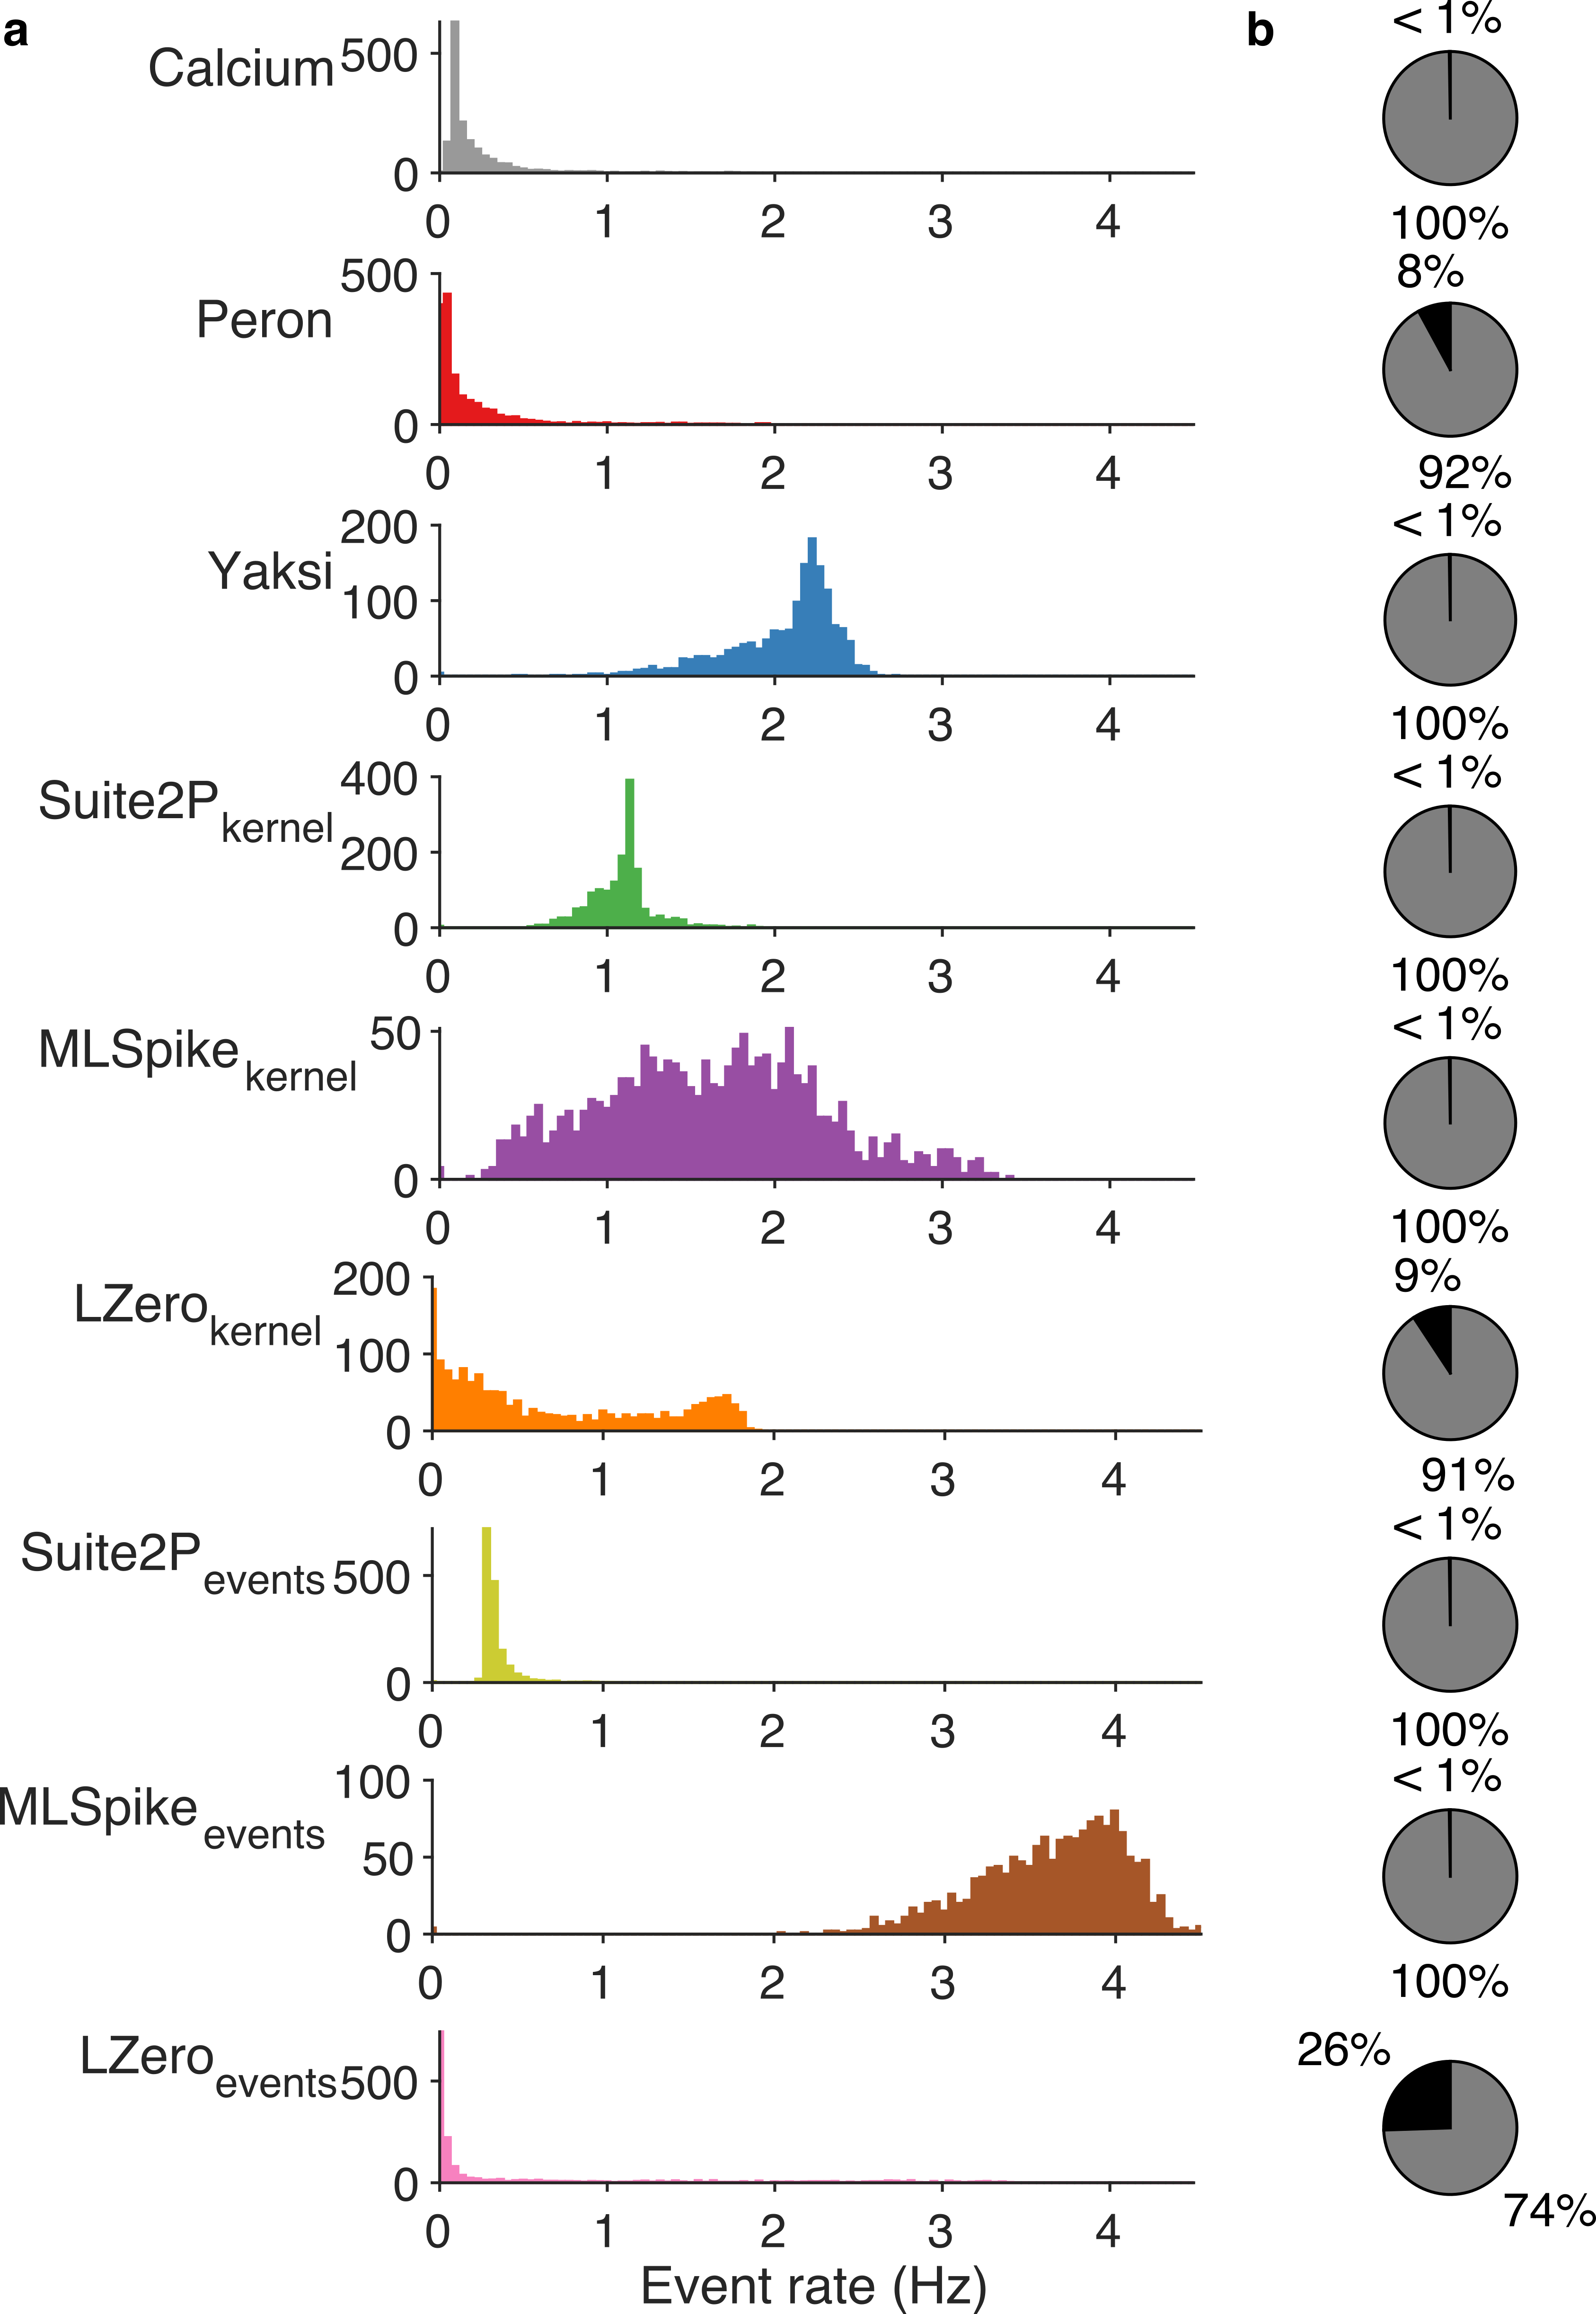
\includegraphics[width=0.8\textwidth]{composite_figs/fig4_event_rate.png}
	\caption{\label{fig:simple_stats} \textbf{Estimates of population-wide event rates vary qualitatively across deconvolution methods.} \\
		(a) The distribution of event rate per neuron across the recorded population, according to each deconvolution method. For raw calcium and the five denoising methods (upper 6 panels), events are detected as fluorescence transients greater in magnitude than three standard deviations of background noise. The discrete deconvolution methods (lower 3 panels) return per frame: a spike count (MLSpike), a binary event detection (LZero), or an event magnitude (Suite2p); these time-series were thus sparse, with most frames empty. \\  
		(b)  Proportion of active (gray) and silent (black) cells for each method. Silent cells are defined following \citep{Peron2015-kd} as those with an event rate less than 0.0083Hz.}
\end{figure*}

We first check how well each approach recovers the basic statistics of neural activity event rates in L2/3 of barrel cortex. Electrophysiology has shown that the distribution of firing rates across neurons in a population is consistently long-tailed, and often log-normal, all across rodent cortex \citep{Wohrer2013-rp}; and L2/3 neurons in barrel cortex are no different \citep{OConnor2010-hd}, with median firing rates less than 1 Hz, and a long right-hand tail of rarer high-firing neurons. We thus expect the calcium event rates or spike rates from our time-series would follow such a distribution. (Event rates for raw calcium, Peron, Yaksi and the continuous (kernel) versions of the data was obtained by thresholding the calcium time-series)

Figure \ref{fig:simple_stats}a shows that the raw calcium and two of the discrete deconvolution methods (Suite2p, LZero) have qualitatively correct distributions of event rates (median near zero, long right-hand tails). The Peron time-series also have the correct distribution of event rates, which is unsurprising as it was tuned to do so. All other methods give qualitatively wrong distributions of spike rates (MLSpike) or event rates (all other methods). There is also little overlap in the distributions of spike rates between the three discrete deconvolution methods. Applying a kernel to their inferred spikes/events shifts rather than smooths the firing rate distributions (Suite2P$_{kernel}$, MLSpike$_{kernel}$, LZero$_{kernel}$), suggesting noise in the deconvolution process is amplified through the additional steps of convolving with a kernel and thresholding.

Cell-attached recordings in barrel cortex have shown that $\sim$26\% of L2/3 pyramidal cells are silent during a similar pole localisation task, with silence defined as emitting fewer than one spike every two minutes \citep{OConnor2010-hd}. For the nine approaches we test here, six estimated the proportion of silent cells to be less than 1\%, including two of the discrete deconvolution methods (Figure \ref{fig:simple_stats}c). For raw calcium and methods returning continuous time-series, raising the threshold for defining events will lead to more silent cells, but at the cost of further shifting the event rate distributions towards zero. Even for simple firing statistics of neural activity, the choice of time-series gives widely differing, and sometimes wrong, results.

\subsection{Inferences of single cell tuning differ widely between raw calcium and deconvolved methods}
We turn now to what we can infer about simple properties of neural coding, and how our choice of deconvolution method can alter those inferences. The decision task facing the mouse (Fig. \ref{fig:peron_setup}a) requires that it moves its whisker back-and-forth to detect the position of the pole, delay for a second after the pole is withdrawn, and then make a choice of the left or right lick-port based on the pole's position (Fig. \ref{fig:peron_setup}b). As the imaged barrel corresponds to the single spared whisker (on the contralateral side of the face), so the captured population activity during each trial likely contains neurons tuned to different aspects of the task. We show here that the number and identity of such task-tuned neurons in the population differ widely between deconvolution methods. 

Following \citealt{Peron2015-qz}, we define a task-tuned cell as one for which the peak in its trial-averaged histogram of activity exceeds the predicted upper limit from shuffled data (Fig.\ref{fig:tuned_cells}a; see Methods). When applied to the raw calcium time-series, close to half the neurons are tuned (Fig.\ref{fig:tuned_cells}a). This is more than double the proportion found for the next nearest method (Yaksi's simple deconvolution), and at least a factor of 5 greater than the proportion of tuned neurons resulting from any discrete deconvolution method, which each report less than 10\% of the neurons are tuned. 

Worse, few neurons are detected as tuned in time-series resulting from multiple methods (Fig.\ref{fig:tuned_cells}b). Only 104 neurons (6.7\%) are labelled as tuned in at least two sets of time-series, and just 21 (1.35\%) are labelled as tuned in all nine. Even separately considering the continuous and discrete time-series, we find only 38 cells are tuned across all six continuous methods, and 25 neurons for all three discrete deconvolution methods (Fig.\ref{fig:tuned_cells}c). Figure \ref{fig:tuned_cells}d illustrates the diversity of detected tuning even amongst the neurons with the greatest agreement between methods.


\begin{figure}
	\centering
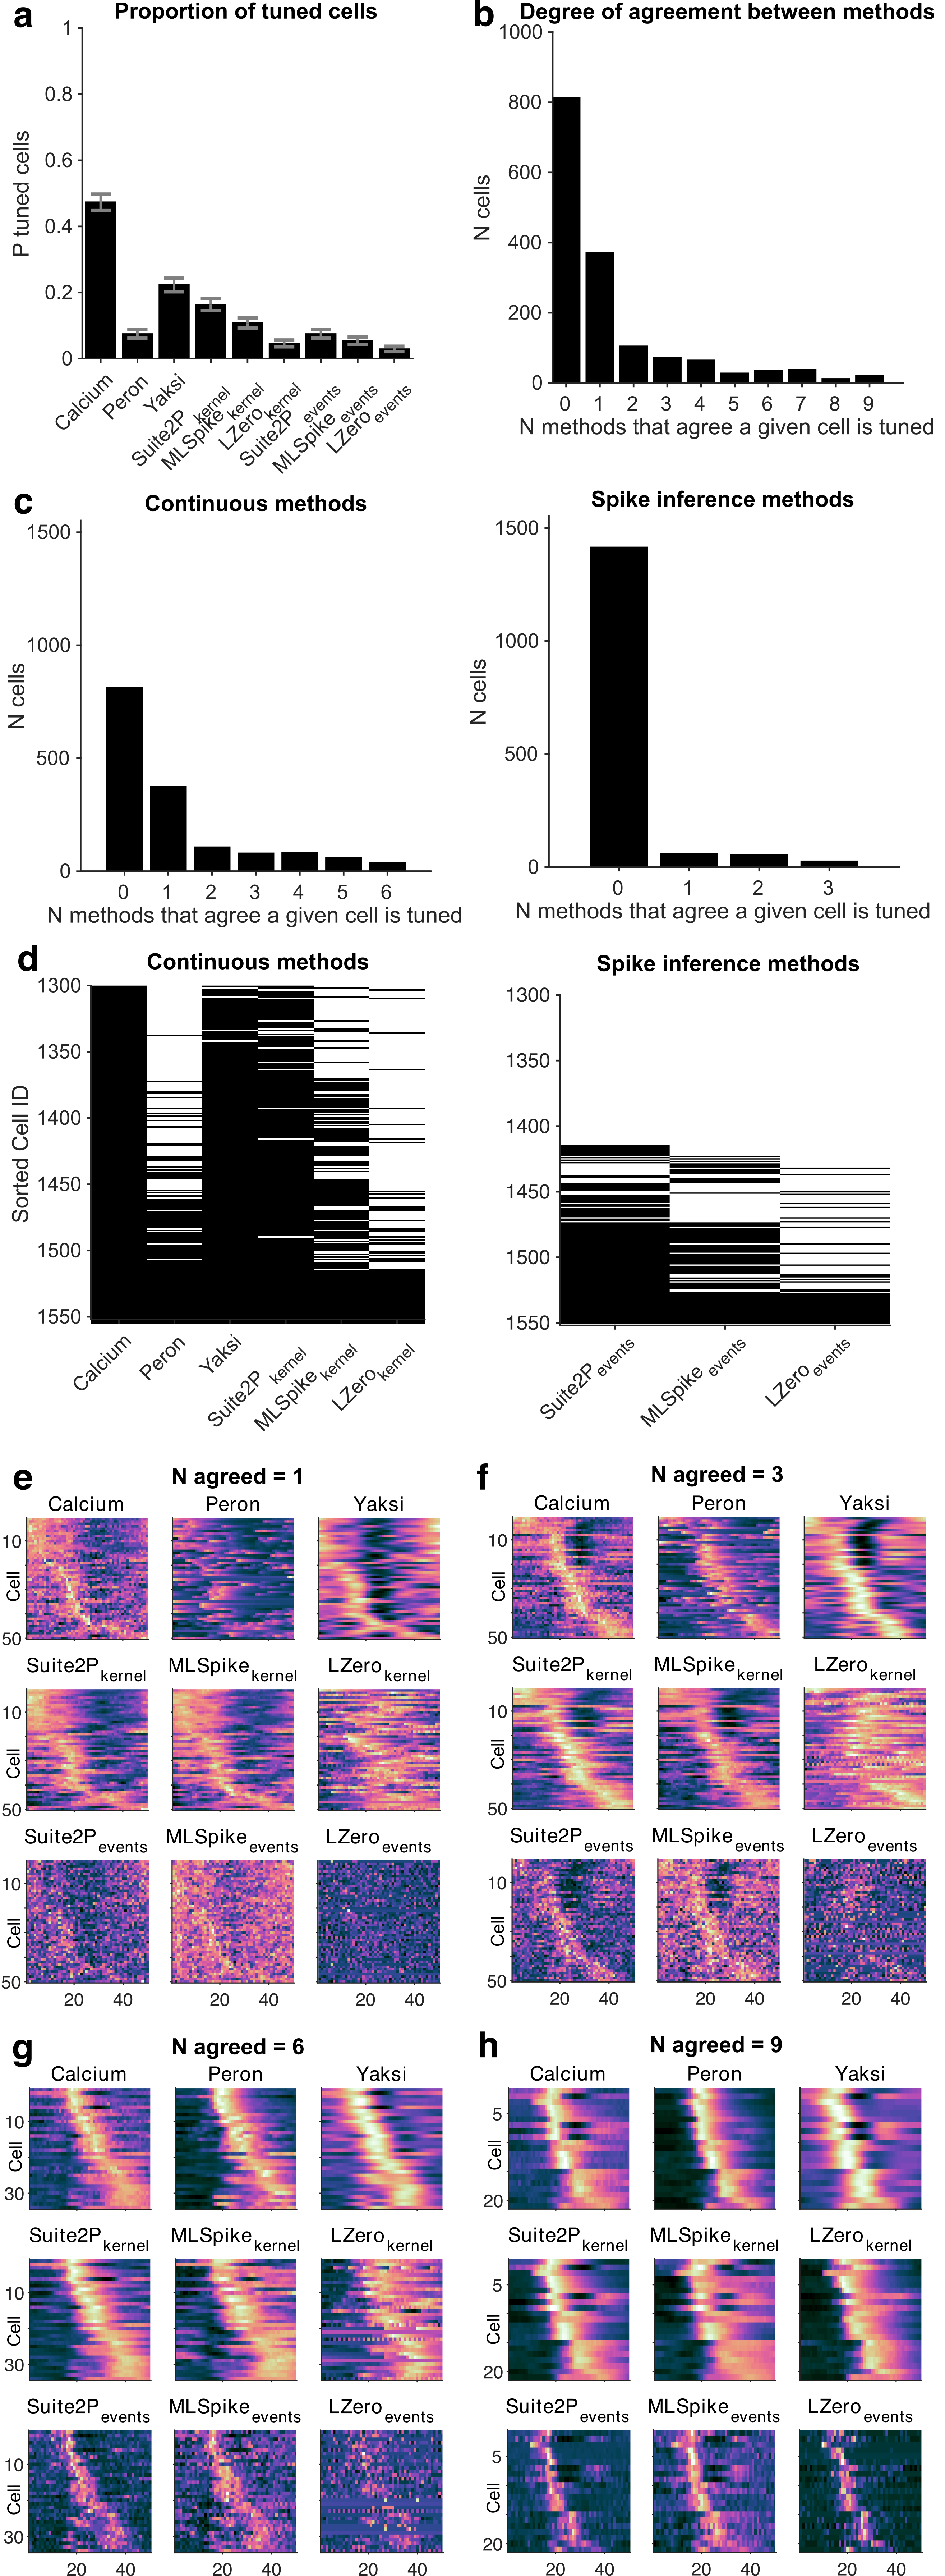
\includegraphics[width=0.45\textwidth]{composite_figs/fig5_tuned_cells.png}
\caption{\label{fig:tuned_cells} \textbf{Inferences of single cell tuning show poor agreement between raw calcium and deconvolution methods, and between methods}. \\
	(a0) Examples of a tuned (left) and non-tuned (right) cell from the raw calcium time-series. X: Data; Y: upper 95\% interval from shuffled data.  \\
	(a) Number of tuned cells per deconvolution method. Error bars are 95\% binomial confidence intervals. \\ 
	(b) Agreement between methods. For each neuron, we count the number of methods (including raw calcium) for which it is labelled as tuned. Bars show the number of cells classified as tuned by exactly $N$ methods. \\
	(c) Similar to (b), but breaking down the cells into: agreement between methods (raw or denoising) resulting in continuous signals (left panel); and agreement between discrete deconvolution methods (right panel). \\ 
	(d) Comparison of cell tuning across methods. Each row shows whether that cell is tuned (black) or not (white) under that deconvolution method. Cells are ordered from bottom to top by the number of methods that classify that cell as tuned. \\
	(e-h) Identifying robust cell tuning. Panel groups (e) to (h) show cells classed as tuned by increasing numbers of deconvolution methods. Each panel within a group plots one cell's normalised (z-scored) trial-average histogram per row, ordered by the time of peak activity. The first panel in a group of 9 shows histograms from raw calcium signals; each of the 8 subsequent panel shows trial-average histograms for the same cells, but following processing by each of the eight deconvolution methods. [Q: How were the neurons chosen?]
}
\end{figure}

These results suggest that raw calcium alone over-estimates tuning in the population, but also that there can be substantial disagreement between deconvolution methods. One solution for robust detection of tuned neurons is to find those agreed between the raw calcium time-series and more than one deconvolution method. In Figure \ref{fig:tuned_cells}e-h, we show how increasing the number of methods required to agree on a neuron's tuned status creates clear agreement between time-series processed with all methods, even if a particular method did not reach significance for that cell. Even requiring agreement between the raw calcium and just two other methods is enough to see tuning of many cells. The identification of unambiguously task-tuned cells could thus be achieved by triangulating the raw calcium with the output of multiple deconvolution methods.

In the pole detection task considered here, neurons tuned to pole contact are potentially crucial to understanding the sensory information used to make a decision. Touch onset is known to drive a subset of neurons to spike with short latency and low jitter \citep{OConnor2010-hd, Hires2015-by}. Detecting such rapid, precise responses in the slow kinetics of calcium imaging is challenging, suggesting discrete-deconvolution methods might be necessary to detect touch-tuned neurons. To test this, in each of the 9 sets of time-series we identify touch-tuned neurons by a significant peak in their tough-triggered activity (Fig \ref{fig:touch_triggered}a). Figure \ref{fig:touch_triggered}b shows that, while all data-sets have touch-tuned neurons, the number of such neurons differs substantially between them. And rather than being essential, discrete deconvolution methods disagree strongly on touch-tuning, with MLSpike (events) finding 45 touch-tuned neurons and LZero (events) finding one. Thus our inferences of the coding of task-wide or specific sensory events crucially depends on our choice of calcium imaging time-series.

\begin{figure}
	\centering
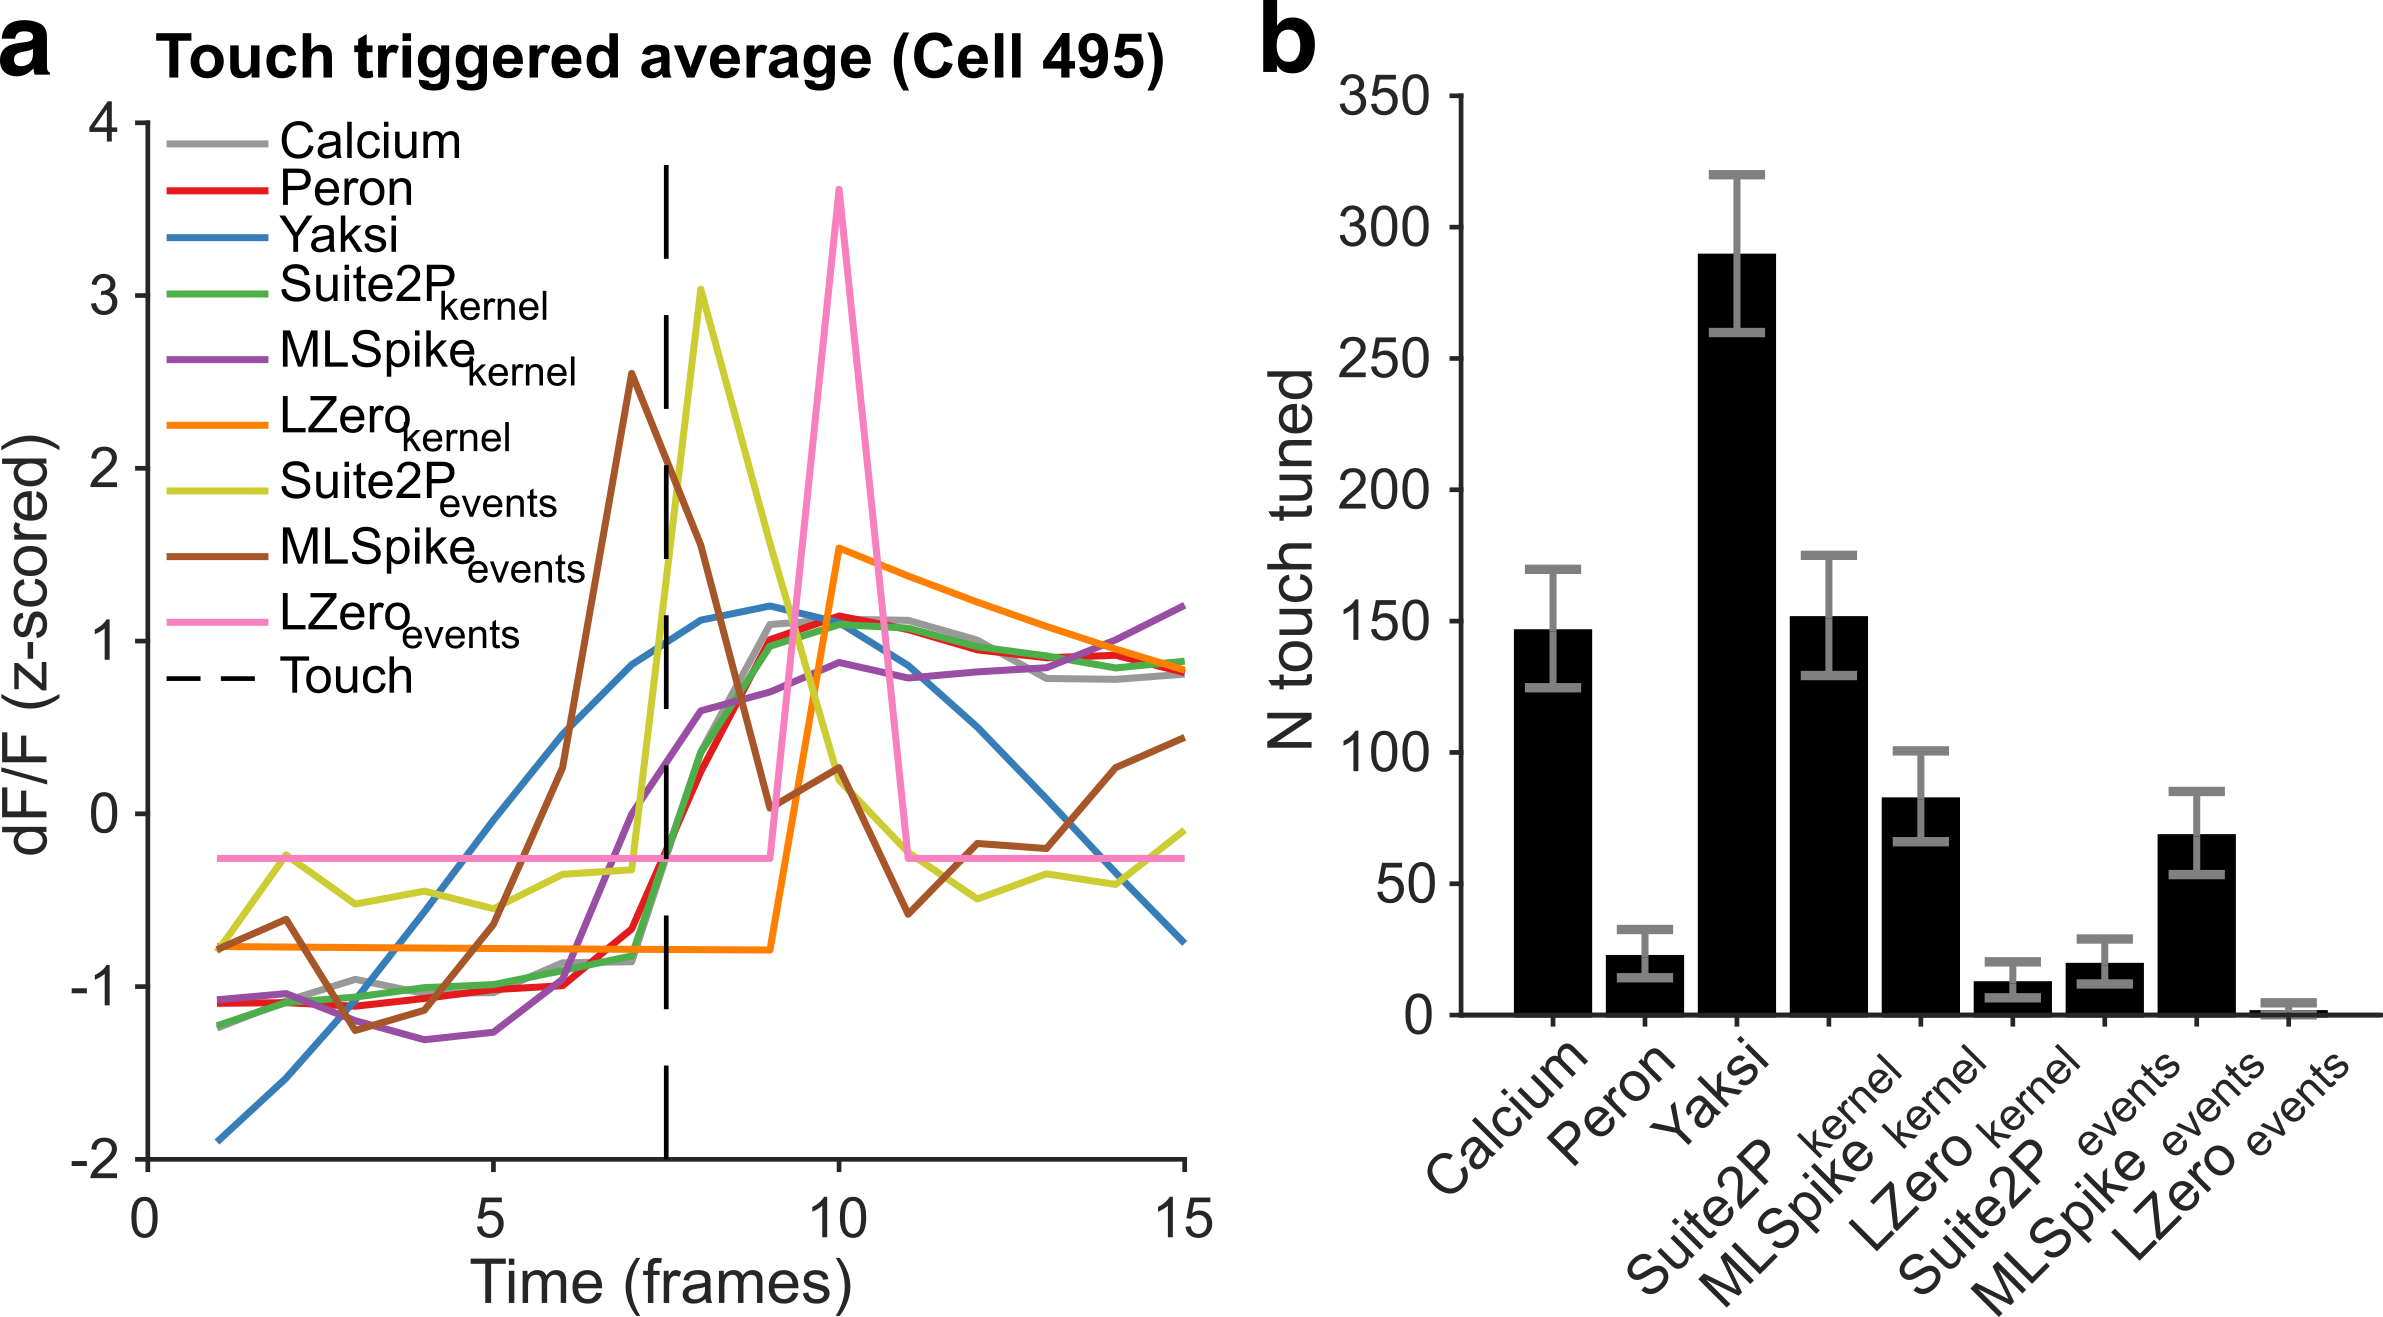
\includegraphics[width=0.7\textwidth]{composite_figs/fig6_touch_tuning}
\caption{\label{fig:touch_triggered} \textbf{Touch-triggered neuron responses}. \\ 	
	(a) Touch-triggered average activity from one neuron, across all deconvolution methods. The dotted line is the imaging frame in which the whisker touched the pole. \\
	(b) Number of touch-tuned cells across deconvolution methods. A cell is classed as touch-tuned if its peak touch-triggered activity is significantly greater than shuffled data. Error bars are Jeffreys intervals}
\end{figure}


\subsection{Inconsistent recovery of population correlation structure across deconvolution approaches}
The high yield of neurons from calcium imaging is ideal for studying the dynamics and coding of neural populations \citep{Harvey2012-bh,Huber2012-mi,Kato2015-sb}. Many analyses of populations start from pairwise correlations between cells, whether as measures of a population's synchrony or joint activity, or as a basis for further analyses like clustering and dimension reduction \citep{Cunningham2014-vd}. We now show how our inferences of population correlation structure also depend strongly on the choice of deconvolution method.

Figure \ref{fig:cxy_dist}a shows that the distributions of pairwise correlations qualitatively differ between the sets of time-series we derived from the same calcium imaging data. The considerably narrower distributions from the discrete deconvolution time-series compared to the others is expected, as these time-series are sparse. Nonetheless, there are qualitative differences within the sets of discrete and continuous time-series. Some distributions are approximately symmetric, with broad tails; some asymmetric with narrow tails; the correlation distribution from the Peron method time-series is the only one with a median below zero. These qualitative differences are not due to noisy estimates of the pairwise correlations: for all our sets of time-series the correlations computed on a sub-set of time-points in the session agree well with the correlations computed on the whole session (Figure \ref{fig:cxy_dist}b). Thus pairwise correlation estimates for each method are stable, but their distributions differ between methods.

\begin{figure*}
	\centering
	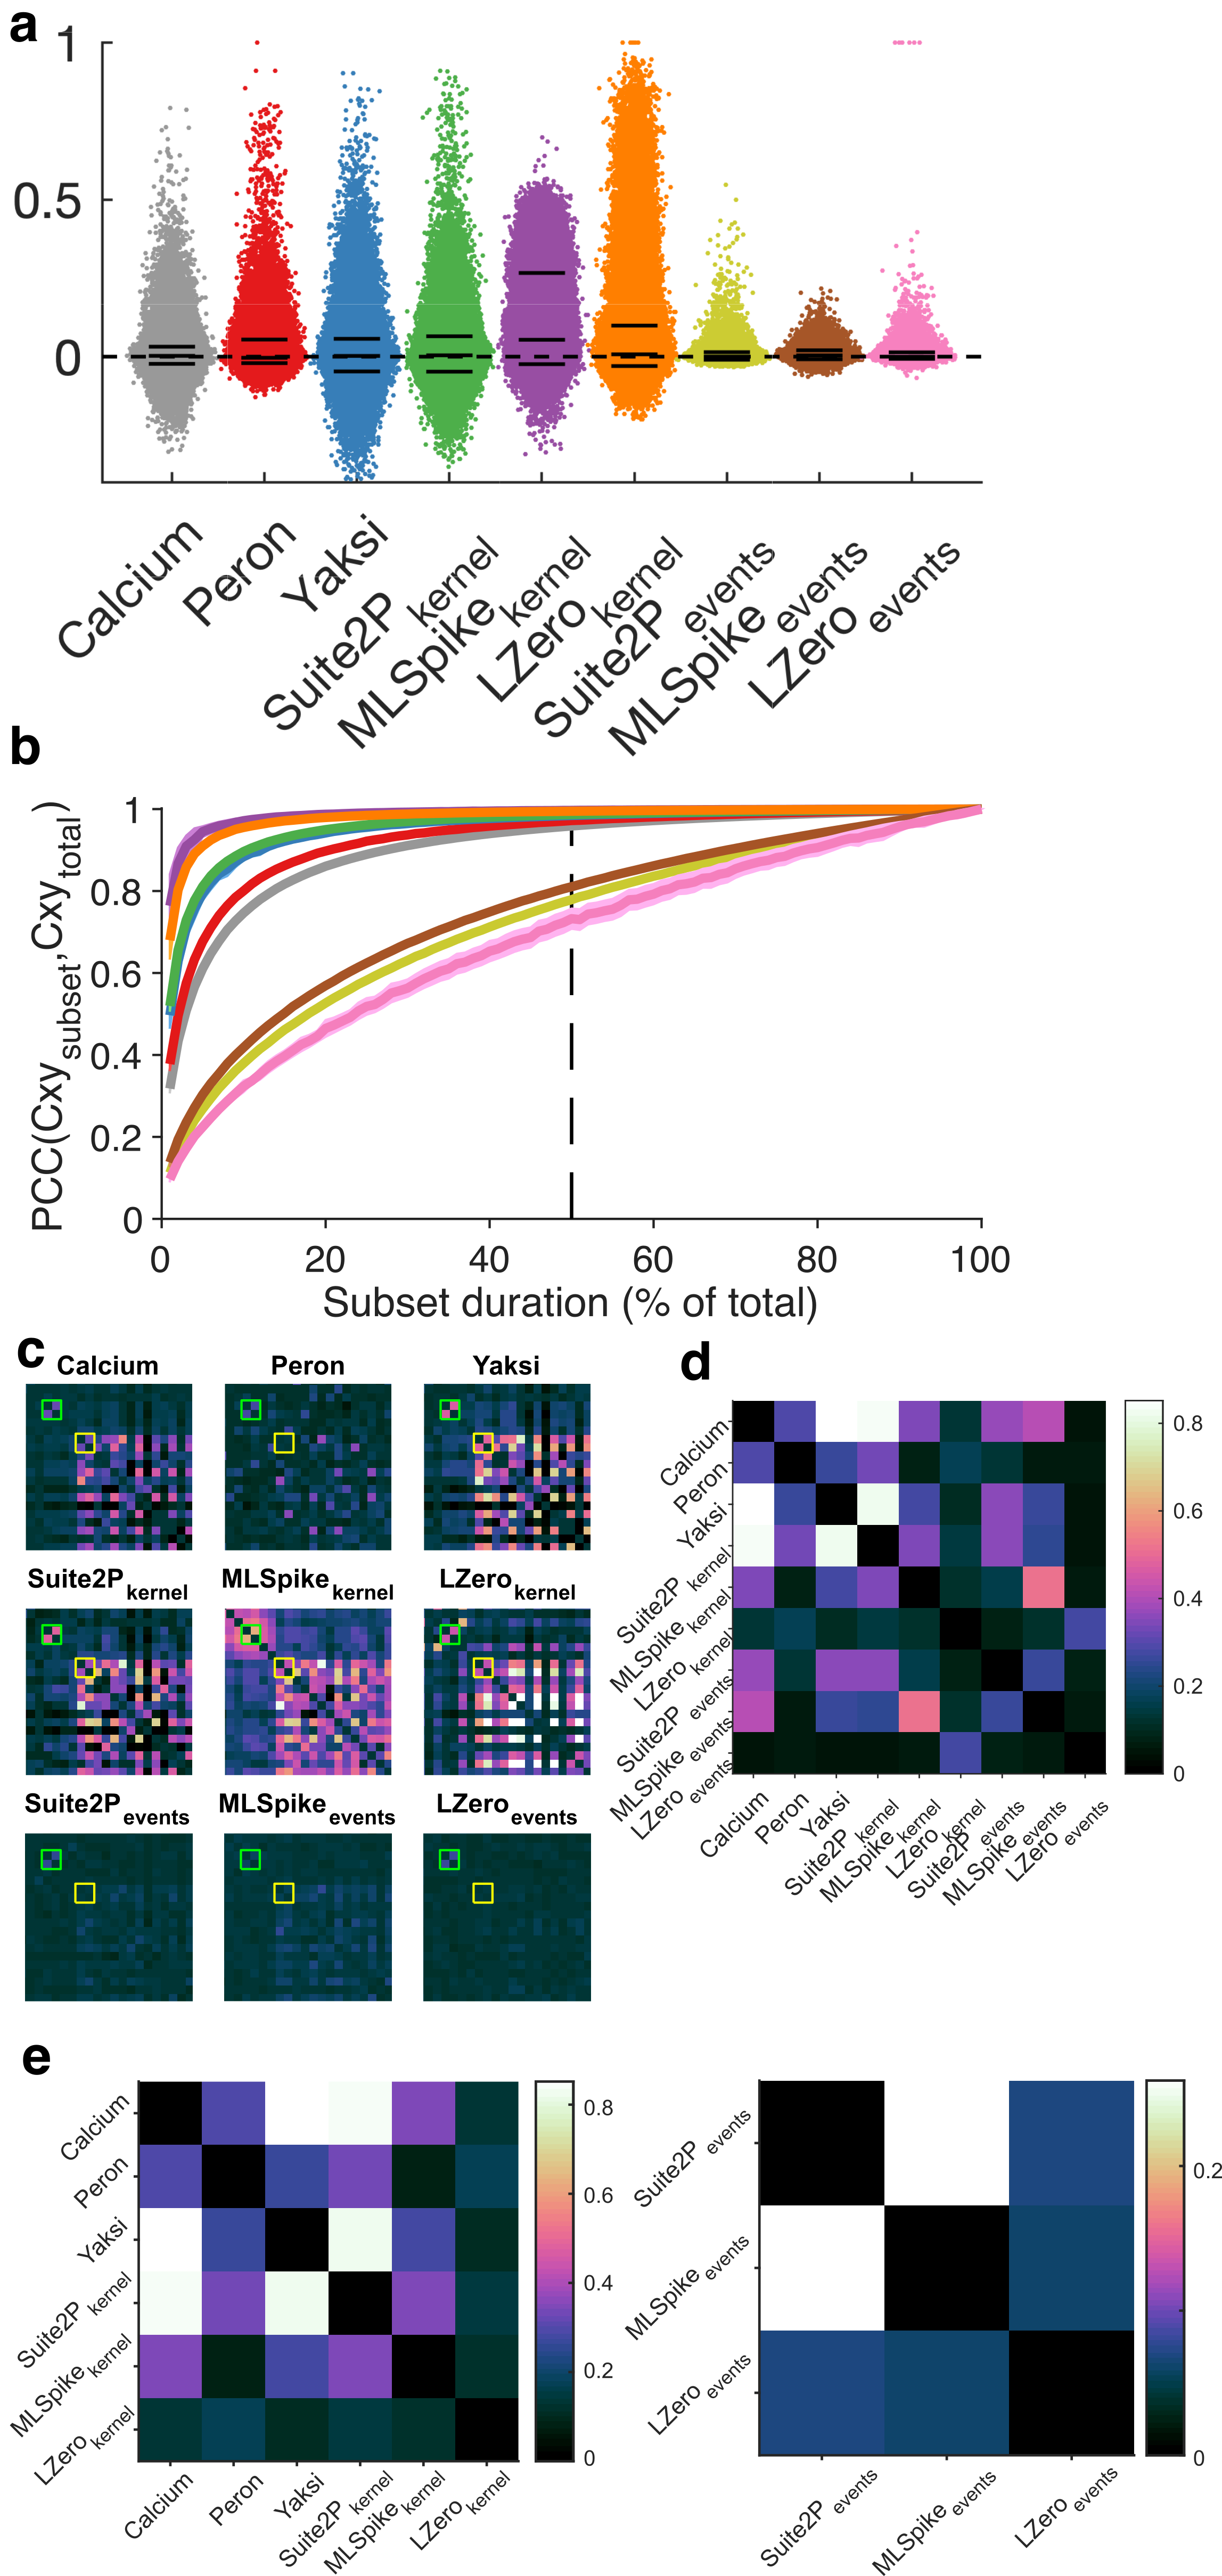
\includegraphics[width=0.5\textwidth]{composite_figs/fig7_correlations}
	\caption {\label{fig:cxy_dist} \textbf{Effects of deconvolution on pairwise correlations between neurons}. \\ 
		(a) Distributions of pairwise correlations between all cells, for each deconvolution method (one dot per cell pair, x-axis jitter added for clarity). Solid black lines are 5th, 50th and 95th percentiles. \\
		(b) Stability of correlation structure in the population. We quantify here the stability of the pairwise correlation estimates, by comparing the correlation matrix constructed on the full data ($Cxy_{total}$) to the same matrix constructed on a subset of the data ($Cxy_{subset}$). Each data-point is the mean correlation between $Cxy_{total}$ and $Cxy_{subset}$; one line per deconvolution method. Shaded error bars are one standard deviation of the mean across 100 random subsets.\\
		(c) Examples of qualitatively differing correlation structure across methods. Each panel plots the pairwise correlations for the same 50 neurons on the same colour scale. As examples, we highlight two pairs of cells: one consistently correlated across different methods (green arrow and boxes); the other not (yellow arrow and boxes). \\
		(d) Comparison of pairwise correlation matrices between deconvolution methods. Each square is the Spearman's rank correlation between the full-data correlation matrix for that pair of methods. \\
		(e) as in (d), but split to show continuous methods (left) or discrete deconvolution methods (right).
	}
\end{figure*}
 
Looking in detail at the full correlation matrix shows that even for methods with similar distributions, their agreement on correlation structure is poor. Some neuron pairs that appear correlated from time-series processed by one deconvolution method are uncorrelated when processed with another method (Figure \ref{fig:cxy_dist}c). Over the whole population, the correlation structure obtained from the raw calcium, Yaksi and Suite2p (kernel) time-series all closely agree, but nothing else does (Figure \ref{fig:cxy_dist}d): the correlation structure obtained from LZero agrees with nothing else; and the discrete deconvolution methods all generate dissimilar correlation structures (Figure \ref{fig:cxy_dist}e). Our inferences about the extent and identity of correlations within the population will differ qualitatively depending on our choice of imaging time-series.


\subsection{Deconvolution methods show the same population activity is both low and high dimensional}

Dimensionality reduction techniques, like principal components analysis (PCA), allow researchers to make sense of large scale neuroscience data \citep{Chapin1999-lf,Briggman2005-ht, Churchland2012-jq, Harvey2012-bh, Cunningham2014-vd,Kobak2016-xy}, by reducing the data from $N$ neurons to $d < N$ dimensions. Key to such analyses is the choice of $d$, a choice guided by how much of the original data we can capture. To assess such inferences of population dimensionality, we apply PCA to our 9 sets of imaging time-series to estimate the dimensionality of the imaging data (which for PCA is the variance explained by each eigenvector of the data's covariance matrix). 

Figure \ref{fig:dimensionality}a plots for each deconvolution method the cumulative variance explained when increasing the number of retained dimensions. Most deconvolution methods qualitatively disagree with the raw calcium data-set on the relationship between dimensions and variance. This relationship is also inconsistent across deconvolution methods; indeed the discrete deconvolution methods result in the shallowest (MLSpike$_{events}$) and amongst the steepest (LZero$_{events}$) relationships between increasing dimensions and variance explained. The number of dimensions required to explain 80$\%$ of the variance in the data ranges from $d=125$ (Peron) to $d=1081$ (MLSpike$_{events}$), a jump from 8$\%$ to 70$\%$ of all possible dimensions (Fig \ref{fig:dimensionality}b). Thus we could equally infer that the same L2/3 population activity is low dimensional ($<$10$\%$ dimensions required to explain 80$\%$ of the variance) or high-dimensional ($>$50$\%$ of dimensions required) depending on our choice of imaging time-series. 

\begin{figure}[h!]
	\centering
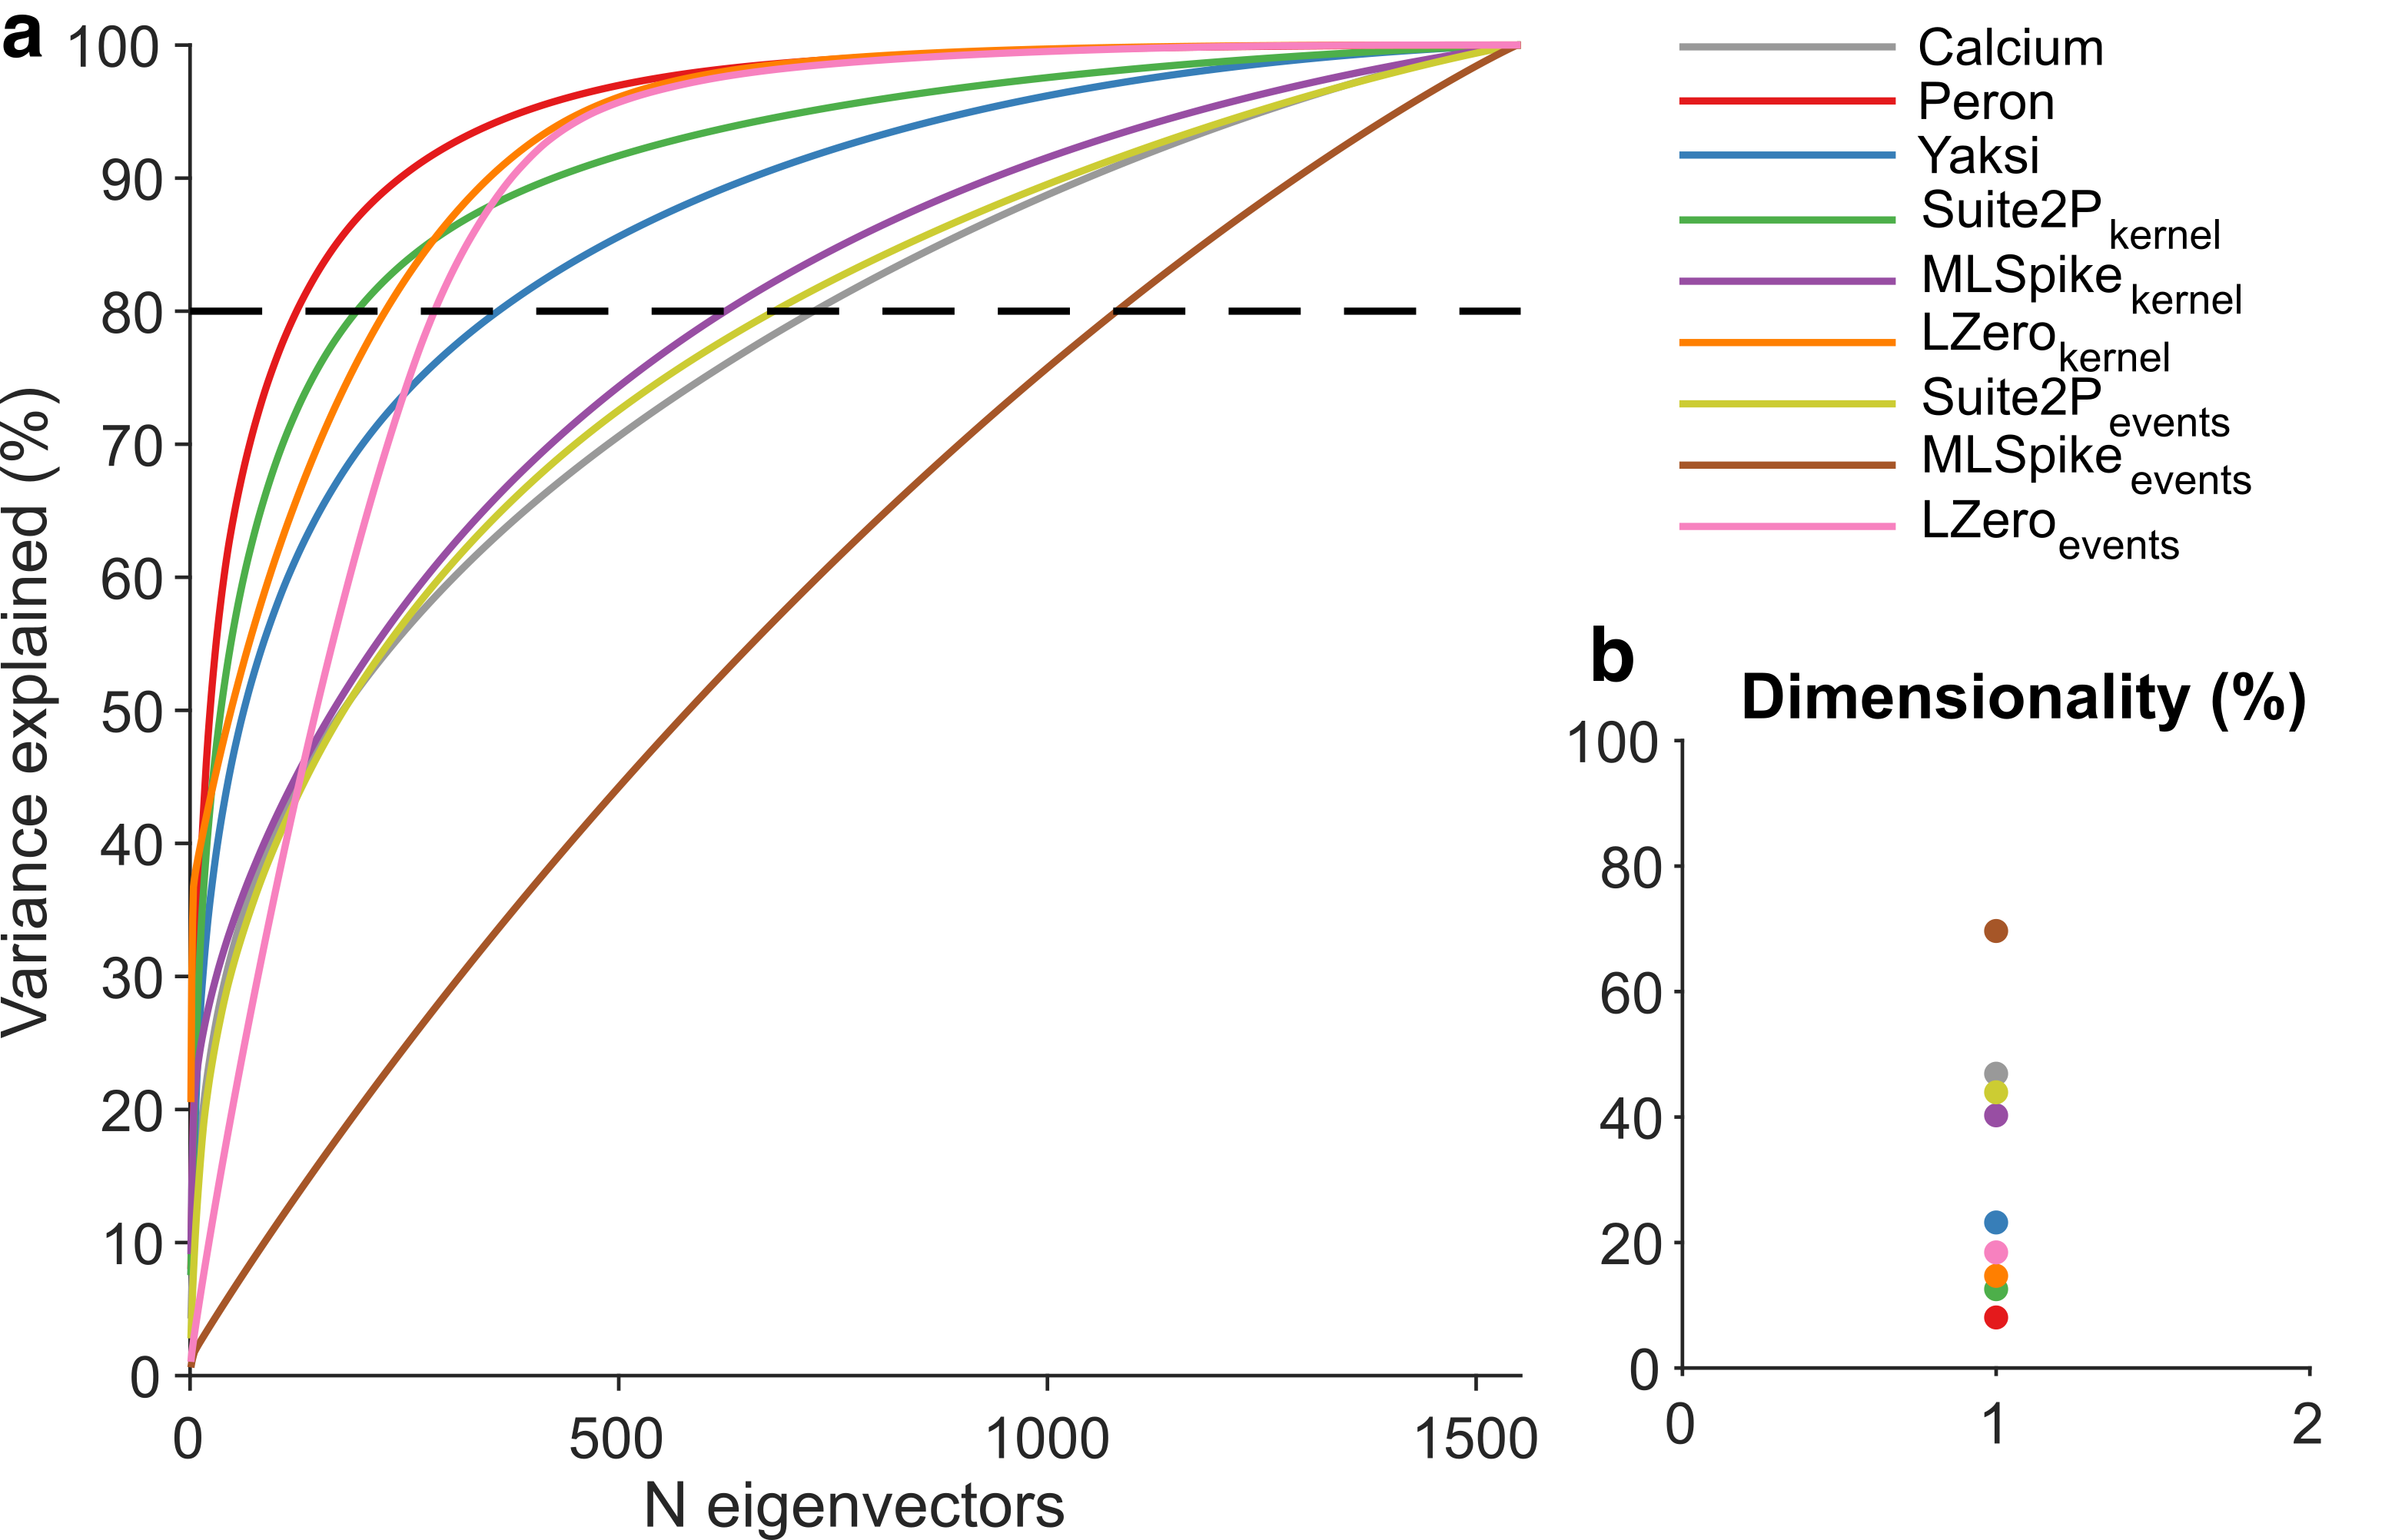
\includegraphics[width=0.8\textwidth]{composite_figs/fig8_dimensionality}
\caption{\label{fig:dimensionality} \textbf{Dimensionality of population activity.} \\
(a) Cumulative variance explained by each dimension of the data’s covariance matrix, one line per deconvolution method. Dimensions are obtained from principal components analysis, and are ordered by decreasing contribution to the total variance explained. Dashed line is the 80\% threshold used in panel (b). \\
(b) Proportion of dimensions required to explain 80$\%$ of the variance in the data.}
\end{figure}



\newpage
\section{Discussion}
Imaging of somatic calcium is a remarkable tool for capturing the simultaneous activity of hundreds to thousands of neurons. But the time-series of each neuron's calcium fluorescence is inherently noisy and non-linearly related to its spiking. We sought here to address how our choice of corrections to these time-series -- to use them raw, deconvolve them into continuous time-series, or deconvolve them into discrete events -- affect the quality and reliability of the scientific inferences drawn.

Our results show the choice qualitatively changes the potential scientific inferences we draw about neural activity, coding, and correlation structure. We consistently observe that the analysis results differ sharply between the raw calcium and most, if not all, of the processed time-series. However, the deconvolved time-series also consistently disagreed with each other, even between methods of the same broad class (continuous or discrete time-series). 

\subsection{Accurate discrete deconvolution is possible, but sensitive}
We find much that is encouraging. In fitting discrete deconvolution methods to ground-truth data, we found they can in principle accurately recover neural activity. A caveat here is that the choice of metric for evaluation and fitting of parameters is of critical importance. The widely-used Pearson correlation coefficient is a poor choice of metric as it returns inconsistent results with small changes in algorithm parameters, and leads to poor estimates of simple measures such as firing rate when used across methods and sampling rates. By contrast, the Error Rate metric \citep{Deneux2016-gu, Victor1996-cg} resulted in excellent recovery of ground-truth spike trains. Other recently developed methods for comparing spike-trains based on information theory \citep{Theis2016-ee} or fuzzy set theory \citep{Reynolds2018-yh}, may also be appropriate. 

However, while good estimates of neural activity can be achieved with modern discrete deconvolution methods \citep{Berens2018-su, Pachitariu2018-cj}, the best parameters vary substantially between cells, and small changes in analysis parameters result in poor performance. This variation and sensitivity of parameters played out as widely-differing results between the three discrete deconvolution methods in analyses of neural activity, coding, and correlation structure.

\subsection{Choosing parameters for deconvolution methods} 
A potential limitation of our study is that we use a single set of parameter values for each discrete deconvolution method applied to the population imaging data from barrel cortex. But then our situation is the same as that facing any experimentalist: in the absence of ground-truth, how do we set the parameters? Our solution here was to use the modal parameter values from ground-truth fitting, as these values are candidates for the most general solutions. We also felt these were a reasonable choice for the population imaging data from barrel cortex, given that the ground-truth recordings came from the same species (mouse) in the same layer (2/3) of a different bit of primary sensory cortex (V1). 
% Choosing the modal parameter values meant that the three methods effectively equivalent between methods; but still led to some striking differences in their results. 

Rather than use the most general parameters values, another solution would be to tune the parameters to obtain known gross statistics of the neural activity. This was the approach used by Peron and colleagues \citep{Peron2015-kd} to obtain the denoised “Peron” time-series we included here. But as we’ve seen, this approach can lead to its own problems: for example, in the Peron time-series, it created a distributions of correlations that differed from any other set of time-series. Indeed, finding good parameter values may be an intractable problem, as it is possible each neuron requires individual fitting, to reflect the combination of its expression of fluorescent protein, and its particular non-linearity between voltage and calcium. 

\subsection{Ways forward}
% Choice of method will constrain interpretations. Peron approach to sparsify data; this introduced shift in pairwise correlations. But for that paper, only single neuron dynamics were assessed.

The simplest solution to the inconsistencies between different forms of time-series is to triangulate them, and take the consensus across their results. For example, our finding of a set of tuned neurons across multiple methods is strong evidence that neurons in L2/3 of barrel cortex are responsive across the stages of the decision task. Further examples of such triangulation in the literature are rare; Klaus and colleagues \citep{Klaus2017-wn} used two different pipelines to derive raw $\Delta F/F$ of individual neurons from one-photon fibre-optic recordings in the striatum, and replicated all analyses using the output of both pipelines. Our results encourage the further use of triangulation to create robust inference: obtaining the same result in the face of wide variation increases our belief in its reliability \citep{Munafo2018-ab}.

There are caveats to using triangulation. For single neuron analyses, triangulation inevitably comes at the price of reducing the yield of neurons to which we can confidently assign roles. A further problem for triangulation is how to combine more complex analyses, such as pairwise correlations; the alternative is to rely on qualitative comparisons.

Many studies use the raw calcium signal as the basis for all their analyses \citep{Harvey2012-bh, Huber2012-mi} [cite others], perhaps assuming this is the least biased approach. Our result show this is not so: the discrepancy between raw and deconvolved calcium on single neuron coding suggests an extraordinary range of possible results, from about half of all neurons tuned to the task down to less 5 percent. The qualitative conclusion -- there is coding -- is not satisfactory. Thus our results should not be interpreted as a call to abandon deconvolution methods; rather they serve to delimit how we can interpret their outputs. 

Instead, we need deconvolution solved: as sensors with faster kinetics (though fundamentally limited by kinetics of calcium release itself) and higher signal-to-noise ratios are developed \citep{Badura2014-ub,Dana2016-yg,Dana2019-mz}, so the accuracy and robustness of de-noising and deconvolution should improve; and as the neuron yield continues to increase \citep{Stringer2019-ze,Ahrens2013-wm}, so the potential for insights from inferred spikes or spike-driven events grows. Developing further advanced deconvolution algorithms will harness these advances, but are potentially always limited by the lack of ground-truth to fit their parameters. Our results may provide impetus for a different direction of research, focussing on how we can get consensus among the output of different algorithms, and thus provide robust scientific inferences about neural populations.

\clearpage
\section{Methods}
\subsection*{Ground truth data}
Ground truth data was accessed from \href{http://crcns.org/data-sets/methods/cai-1}{crcns.org} \citep{Svoboda2015-ym}, and the experiments have been described previously \citep{Chen2013-nv}. Briefly, mouse visual cortical neurons expressing the fluorescent calcium reporter protein GCaMP6s were imaged with two-photon microscopy at 60Hz. Loose-seal cell-attached recordings were performed simultaneously at 10kHz. The data-set contains twenty one recordings from nine cells.


\subsection*{Population imaging data description}
Population imaging data was accessed from \href{https://crcns.org/data-sets/ssc/ssc-2}{crcns.org} and have been described previously \citep{Peron2015-kd}. Briefly, volumetric two photon calcium imaging of primary somatosensory cortex (S1) was performed in awake head-fixed mice performing a whisker-based object localisation task. In the task a metal pole was presented on one of two locations and mice were motivated with fluid reward to lick at one of two lick ports depending on the location of the pole following a brief delay. Two photon imaging of GCaMP6s expressing neurons in superficial S1 was performed at 7Hz. Images were motion corrected and aligned, before regions of interest were manually set and neuropil-subtracted. A single recording from this dataset was used for population analysis. The example session had 1552 neurons recorded for a total of 23559 frames (56 minutes).


\subsection*{List of deconvolution methods}

\subsubsection*{MLSpike}
\texttt{MLSpike} \citep{Deneux2016-gu} was accessed from \href{https://github.com/mlspike}{https://github.com/mlspike}. MLSpike uses a model-based probabilistic approach to recover spike trains in calcium imaging data by taking baseline fluctuations and cellular properties into account. Briefly, 
MLSpike implements a model of measured calcium fluorescence as a combination of spike-induced transients, background (photonic) noise and drifting baseline fluctuations. A maximum likelihood approach determines the probability of the observed calcium at each time step given an inferred spike train generated through a particular set of model parameters. MLSpike returns a maximum a posteriori spike train (as used here), or a spike probability per time step. MLSpike also returns an estimate of the drifting background fluorescence which is ignored in this work. 

MLSpike has a number of free parameters, of which we optimise three: $A$, the magnitude of fluorescence transients caused by a single spike; $tau$, calcium fluorescence decay time; $sigma$, background (photonic) noise level. MLSpike also has parameters for different calcium sensor kinetics (for OBG, GCaMP3, GCaMP6 and so on) which we fix to default values for GCaMP6. 

For our analysis of event rate MLSpike's spike train was counted (mean event count per second), and for subsequent analyses was converted to a dense array of spike counts per imaging frame.

%(\emph{TO DO ?: We show results for both denoted MLSpike$_{events}$ and MLSpike$_{pspike}$ in Supplement})


\subsubsection*{Suite2P}
\texttt{Suite2P} \citep{Pachitariu2016-ui,Pachitariu2018-cj} was accessed from \href{https://github.com/cortex-lab/Suite2P}{https://github.com/cortex-lab/Suite2P}. Suite2P was developed as a complete end-to-end processing pipeline for large scale 2-photon imaging analysis - from image registration to spike extraction and visualization - of which we only use the spike extraction step. The spike deconvolution of Suite2P uses a sparse non-negative deconvolution algorithm, greedily identifying and removing calcium transients to minimise the cost function 

\[C = \|F - s*k\|^2,\]

where the cost $C$ is the squared norm of fluorescence $F$ minus a reconstruction of that signal comprising a sparse array of spiking events $s$ multiplied by a parameterised calcium kernel $k$. The kernel was parameterised following defaults for GCaMP6s (exponential decay of 2 seconds, though it has been shown the precise value of this parameter does not affect performance for this method \citep{Pachitariu2018-cj}. 

Suite2P has a further free parameter which sets the minimum spike event size, the $Threshold$, which determines the stopping criteria for the algorithm.

Elements of $s$ are of varying amplitude corresponding to the amplitude of the calcium transients at that time.  For ground truth firing rate analysis we are interested in each algorithm's ability to recover spike trains, therefore we treat each event as a `spike' and optimise the algorithm appropriately. For our analysis of event rate Suite2P's event train was counted (mean event count per second), and for subsequent analyses was converted to a dense array of varying amplitude events (i.e. $s$) per imaging frame.

%\noindent and our own notes on the spike detection algorithm are here:\\
%
%\noindent \href{https://drive.google.com/open?id=1NeQhmoRpS-x8R0e84w3TqkUR1PNMXiem6ZIjJta-U7A}{https://drive.google.com/open?id=1NeQhmoRpS-x8R0e84w3TqkUR1PNMXiem6ZIjJta-U7A}.



\subsubsection*{LZero}
The method we refer to as \texttt{LZero} was written in Matlab based on an implementation in $R$ accessed at \href{https://github.com/jewellsean/LZeroSpikeInference}{https://github.com/jewellsean/LZeroSpikeInference}. A full description is available in the paper of \citet{Jewell2018-cx}. Briefly, in LZero spike detection is cast as a change-point detection problem, which could be solved with an $l_{0}$ optimization algorithm. Working backwards from the last time point the algorithm finds time points where the calcium dynamics abruptly change from a smooth exponential rise. These change points correspond to spike event times. Spike inference accuracy is assessed similarly to Suite2P by measuring the fit between observed fluorescence and a reconstruction based on inferred spike times and a fixed calcium kernel. 

LZero has two free parameters - $lambda$, a tuning parameter that controls the trade-off between the sparsity of the estimated spike event train and the fit of the estimated calcium to the observed fluorescence; and $scale$, the magnitude of a single spike induced change in fluorescence.

For our analysis of event rate LZero's spike train was counted (mean event count per second), and for subsequent analyses was converted to a dense array of spikes per imaging frame (maximum one spike per imaging frame due to limitations of the algorithm).


%In their paper \citet{Jewell2017-pr} show that the $l_{0}$ solution is better than previously implemented $l_{2}$ solutions, with results much closer to the real spike train ($l_{2}$ solutions tend to overestimate the true firing rate). Details can be found in the paper \citep{Jewell2017-pr}.

%\noindent Link: \href{https://arxiv.org/abs/1703.08644}{https://arxiv.org/abs/1703.08644}

\subsubsection*{Yaksi}
\texttt{Yaksi} is an implementation of the deconvolution approach of \citet{Yaksi2006-ic}. The fluorescence time series is low-pass filtered ($4^{\text{th}}$ order butterworth filter, 0.7Hz cutoff) to remove noise before having a calcium kernel (exponential decay of 2 seconds, as used in Suite2P and LZero above) linearly deconvolved out of the signal using Matlab's {\tt deconv} function. The output of Yaksi is a continuous signal approximating spike density per unit time.

\subsubsection*{Peron events}
\texttt{Peron events} refer to the de-noised calcium event traces detailed in the original \cite{Peron2015-kd} paper. Here a version of the `peeling' algorithm \citep{Lutcke2013-wu} was developed, a template-fitting algorithm with variable decay time constants across events and cells. This algorithm was tuned by the authors to generate a low number of false positive detections (a rate of 0.01Hz) on ground truth data, matching firing rate statistics from cell-attached electrophysiology and leading to a hit rate of 54$\%$. The output for analysis is a continuous signal approximating de-noised calcium concentration per unit time.

\subsubsection*{$Events$ and $kernel$ versions of spike inference methods}
Where a spike inference method returns spike counts per time point, these are plotted as Method$_{events}$. To compare to other methods that return a de-noised dF/F or firing rate estimates, these event traces are convolved with a calcium kernel and plotted as Method$_{kernel}$. The kernel used is consistent with that used as a default for GCaMP6s in MLSpike, Suite2P and LZero, namely an exponential decay of two seconds duration normalised to have an integral of 1.


\subsection*{Ground truth spike train metrics}
% NB. script that generates these results is deconv_downsample.m
Pearson correlation coefficient was computed between the ground truth and inferred spikes (MLSpike) or events (Suite2P, LZero) following convolution of both with a gaussian kernel (61 samples wide, 1.02 seconds). 

Error Rate was computed between the ground truth and inferred spikes/events using the \cite{Deneux2016-gu} implementation of normalised error rate, derived from \cite{Victor1996-cg} Error Rate (code available \href{https://github.com/MLspike}{https://github.com/MLspike}). Briefly, the error rate is 1 - F1-score, where the F1-score is the harmonic mean of sensitivity and precision \citep{Davis2006-ya},
% ($1 - \frac{N missed spikes}{N total spikes}$) and precision ($1 - \frac{N falsely detected spikes}{N detected spikes}$),

\[sensitivity = 1 - \frac{misses}{total \ spikes},\]

\[precision = 1 - \frac{false \ detections}{total \ detections},\]

\[Error Rate = 1 - 2 \frac{sensitivity \times precision}{sensitivity + precision}.\]

\noindent Hits, misses and false detections were counted with a temporal precision of 0.5 seconds.

\noindent For normalised estimation of errors in firing/event rate we compute,

\[\frac{estimated \ rate - true \ rate}{true \ rate},\]

\noindent where spike/event rates are measured in Hz.

\subsection*{Parameter fitting}
For each method the best parameters for each cell were determined by brute force search over an appropriate range (i.e. at least two orders of magnitude encompassing full parameter ranges used in the original publications for each method). The parameter ranges were explored on a log scale as follows: MLSpike A (0.01:1, 21 values), tau (0.01:5, 21 values), sigma (0.01:1, 21 values); Suite2P Threshold (0.1:100, 13 values);  LZero lambda (0.1:20, 23 values), scale (0.1:20, 23 values). 

The modal best parameters, as determined using Error Rate on downsampled data, were then fixed for the population imaging data analysis. These were: MLSpike A: 0.1995, tau: 1.9686, sigma: 0.0398; Suite2P Threshold: 1.7783; LZero sigma: 0.1; lambda: 3.1623.

% [ARE THESE HAPPENING - if not, delete? 
%  MHE: I do have these data for most tests. I can add them in if needed. 

% In additional tests (\emph{TO DO Supplemental figs, subscript 'PCC'}), the modal best parameters when assessed using correlation coefficent were used, and in the case of MLSpike parameters were additionally hand-tuned using a built-in GUI (\emph{TO DO Supplemental figs, subscript 'hand'})].

\subsection*{Downsampling}
Ground truth calcium data was downsampled from 60Hz to 7Hz in Matlab by up-sampling by 7 - {\tt{interp(ca,7)}} and downsampling the resultant 420Hz signal by 60 as Matlab's downsampling must be done in integer steps.  [??? how was the downsampling done then? By taking every Nth frame from the interpolated data? Or averaging over every approx 8.5 frames of the 60Hz signal?]. {\color{red} Yes by downsampling the interpolated data. Is this not clear from what I've re-written?. The 60Hz signal is upsampled by 7 to 420 Hz, which is then down sampled by a factor of 60 to 7Hz.}


\subsection{Event rate estimation}
Spike inference methods (Suite2P$_{events}$,MLSpike$_{events}$, LZero$_{events}$) return estimated spike times (MLSpike), or event times (Suite2P/LZero) which were converted into mean event rates (Hz) per cell.

The event rate for continuous methods (Calcium, Peron, Yaksi, Suite2P$_{kernel}$, MLSpike$_{kernel}$, LZero$_{kernel}$) for each cell was determined by counting activity/fluorescence transients greater than three standard deviations of the background noise. Background noise was calculated by subtracting a smoothed four-point moving average of the fluorescence from the raw data to result in a 'noise only' trace. This operation was done separately for each cell and each method. Event rate was then computed in Hz. 

[what does this all mean? That each data-point for the background noise was an average over 4 adjacent frames, and the standard deviation of the noise was computed from those data-points? Why smooth the noise? And what segment of the data was treated as "background"? (i.e. how many data-points)? Or does this mean that the whole Ca2+ trace for each cell was smoothed using a 4-frame average (shifting 1 frame?), and the SD of that smoothed signal was used as an estimate of background noise?] {\color{red} No. I have re-written for clarity. I'm trying to isolate the high-frequency noise by subtracting the low-frequency component first. So the df/f is smoothed, and this smoothed signal is subtracted from the original data to leave a noise-only trace. This noise-only trace is what the detection threshold is computed from. Does this logic make sense, and does my explanation now explain what I did?}

Silent cells were defined as cells with event rates below 0.0083Hz (or fewer than one spike per two minutes of recording) as in \cite{OConnor2010-hd}.

\subsection{Task-tuned cells}
Task-tuning was determined for each neuron using the model-free approach of \cite{Peron2015-kd}. Neurons were classed as task-tuned if their peak trial-average activity exceeded the 95th percentile of a distribution of trial-average peaks from shuffled data (10000 shuffles). The shuffle test was done separately for correct lick-left and lick-right trials and cells satisfying the tuning criteria in either case were counted as task-tuned.

Tuned cell agreement was calculated as the number of methods that agreed to the tuning status of a given cell, for all methods and separately for continuous and spike inference methods.

\subsection{Touch-related responses}
Touch-tuned cells were determined by computing touch-triggered average activity for each cell, before calculating whether the data distribution of peak touch-induced activity exceeds the expected activity of shuffled data. In more detail, the time of first touch - between the mouse's whisker and the metal pole - on each trial was recorded. For each touch time, one second of activity (seven data samples) was extracted before and after the frame closest to touch (15 samples total); taking the mean of these gave the average touch response for the cell. To determine whether a cell was touch tuned or not the time of peak touch-triggered average activity was calculated, and a Wilcoxon rank sum test (Benjamini Hochberg corrected, alpha 0.05) between the true data distribution at peak time and a matched random sample of data from the same cell was performed.

[unclear what the pairwise tests were between; the mean activity at the peak time, and a N-length vector of mean activity as the same time obtained from N shuffled datasets?] 
 
 {\color{red} The test was between the distribution around the peak (e.g. 100 values from 100 touches) and a matched random sample of the data (e.g. 100 other points taken at random from that cell's time series.}
 
[Shuffled how many times? Shuffled how?]. 

{\color{red} Not really a shuffle. it's a matched (N data points for N touches, 133 in this case) random sample. I think this is equivalent to a shuffle, no?}

\subsection{Pairwise correlations}
Pairwise correlations (Pearson correlation coefficients, Fig. \ref{fig:cxy_dist}a) were calculated for all pairs of neurons in Matlab (corrcoef) at the data sampling rate (7Hz). 

[State what forms of time-series were correlated - from debugging doc {\color{red} I've put the format of each method in the method description section, and put this section before the analysis sections. Does this address this point appropriately?}]  

Stability of correlation estimates (Fig. \ref{fig:cxy_dist}b) at the recording durations used was assessed by computed the similarity between correlation distributions for the the intact dataset to those from subsets of the dataset. For each deconvolution method, we computed the pairwise correlation matrix using the entire session’s data, as above. We also sampled a subset of time-points (1\%-100\%) of the full dataset at random without replacement and computed a matrix of pairwise correlations for this subset. We then compute the similarity between the total and subset matrices using Pearson’s correlation coefficient. This process was repeated 100 times and the mean (line) and standard deviation (shading) of the 100 repeats were plotted.

\subsection{Correlations between correlation matrices}
Correlations between correlation matrices (Fig. \ref{fig:cxy_dist}c-e) were computed using Spearman's rank correlation between the unique pairwise correlations from each method (i.e. the upper triangular entries of the correlation matrix). % {\tt CXY(find(triu(CXY)))}).

\subsection{Dimensionality}
To determine the dimensionality of each dataset we performed eigendecomposition of the covariance matrix of each dataset. [Computed as per the pairwise correlations above? {\color{red}not sure what you mean? In terms of data format yes...} ] The resultant eigenvalues were sorted into descending order, and the cumulative variance explained plotted, and the number of eigenvectors required to explain 80\% of the variance recorded. % ({\tt cumsum(egs)/sum(egs)})


\bibliographystyle{plainnat}
\bibliography{references}

\end{document}